\chapter{Osnovne algoritamske paradigme}

Prilikom rješavanja računarskih problema često se koriste određeni obrasci razmišljanja i pristupi konstruisanju algoritama. Takvi pristupi nazivaju se \textit{algoritamske paradigme}. Svaka paradigma predstavlja opšti metod za dizajniranje algoritama i može se primijeniti na širok spektar problema.

Prije nego što pređemo na algoritamske paradigme, vrijedi pomenuti da postoje i različite \textit{programske paradigme}, odnosno stilovi programiranja koji određuju način organizacije i pisanja programskog k\^oda. Najpoznatije programske paradigme su:

\begin{itemize}
	\item \textit{imperativno programiranje}, zasnovano na sekvencijalnom izvršavanju naredbi;
	\item \textit{funkcionalno programiranje}, koje naglasak stavlja na funkcije i transformaciju podataka;
	\item \textit{logičko programiranje}, zasnovano na pravilima i zaključivanju;
	\item \textit{objektno orijentisano programiranje}, koje modeluje probleme pomoću objekata i njihovih međusobnih interakcija.
\end{itemize}

Savremeni programski jezici često podržavaju više paradigmi istovremeno, omogućavajući programerima da odaberu pristup koji najbolje odgovara problemu koji rješavaju.

Kada je riječ o algoritmima, različiti problemi zahtijevaju različite strategije dizajniranja. Upravo te strategije nazivamo algoritamskim paradigmama. U nastavku navodimo najvažnije među njima.

\begin{itemize}

	\item \textbf{Rekurzivni algoritmi}
	
	Zasnivaju se na razlaganju problema na manje podprobleme iste prirode. Rješenje se dobija rekurzivnim pozivanjem algoritma sve dok se ne dostigne jedan od baznih slučajeva.
	
	\item \textbf{Algoritmi grube sile} (eng. \textit{brute force})
	
	Zasnivaju se na ispitivanju svih mogućih rješenja dok se ne pronađe ispravno ili optimalno rješenje. Jednostavni su za implementaciju, ali često imaju visoku vremensku složenost.
	
	\item \textbf{Podijeli pa zavladaj} (eng. \textit{divide-and-conquer})
	
	Problem se dijeli na više manjih nezavisnih podproblema koji se rješavaju odvojeno, nakon čega se njihova rješenja kombinuju u rješenje originalnog problema.% Klasični primjeri su Sortiranje spajanjem i Brzo sortiranje.
	
	\item \textbf{Pohlepni algoritmi} (eng. \textit{greedy algorithms})
	
	U svakom koraku donose lokalno najbolje moguće rješenje, uz pretpostavku da će takav izbor dovesti do globalno optimalnog rješenja. Karakterišu ih jednostavnost i mala potrošnja memorije, ali ne garantuju optimalnost za većinu problema.
	
	\item \textbf{Dinamičko programiranje} (eng. \textit{dynamic programming})
	
	Problem se razlaže na podprobleme koji se međusobno preklapaju. Rezultati već riješenih podproblema memorišu se i ponovo koriste, čime se izbjegava višestruko računanje istih vrijednosti.
	
	\item \textbf{Vraćanje unazad} (eng. \textit{backtracking})
	
	Rješenje se gradi postepeno. Kada se ustanovi da trenutno parcijalno rješenje ne može dovesti do validnog rješenja, algoritam se vraća na prethodni korak i pokušava alternativni izbor.
	
	\item \textbf{Randomizirani algoritmi}
	
	U proces odlučivanja uvode element slučajnosti. Često se koriste za ubrzavanje algoritama ili za efikasno rješavanje problema velikih dimenzija.
	
\end{itemize}

Važno je naglasiti da ove paradigme nisu međusobno isključive. U praksi se veoma često kombinuju kako bi se dobili efikasniji algoritmi za rješavanje složenih računarskih problema. U nastavku knjige detaljnije ćemo proučiti nekoliko najvažnijih algoritamskih paradigmi i njihove primjene.\\

%ISHODI UCENJA:
\section*{Ishodi učenja}

Nakon uspješnog savladavanja sadržaja ove glave student će biti u stanju da:

\begin{itemize}
	\item objasni princip rekurzije i razlikuje rekurzivni od iterativnog pristupa rješavanju problema;
	
	\item primijeni algoritme grube sile i osnovne algoritme pretraživanja	na jednostavne probleme;
	
	\item objasni i primijeni paradigmu podijeli pa zavladaj pri razlaganju problema na manje podprobleme;
	
	\item koristi paradigmu vraćanja unazad za sistematsko pretraživanje prostora rješenja i odbacivanje nedopustivih parcijalnih rješenja;
	
	\item objasni princip pohlepnih algoritama i prepozna situacije u kojima lokalno najbolji izbor može voditi ka kvalitetnom ili optimalnom rješenju;
	
	\item primijeni dinamičko programiranje kroz definisanje podproblema,
	rekurentnih relacija i memorisanje već izračunatih rezultata te procijeni
	vremensku i prostornu složenost dobijenog algoritma.
\end{itemize}



\section{Rekurzivni algoritmi}

Rekurzija predstavlja jednu od osnovnih algoritamskih paradigmi. Sama riječ potiče od latinske riječi \textit{recurrere}, što znači \emph{vraćati se}. U programiranju se funkcija naziva \textit{rekurzivnom} ukoliko u svom tijelu direktno ili indirektno poziva samu sebe.

Osnovna ideja rekurzije sastoji se u tome da se problem postepeno svodi na manje podprobleme iste prirode. Svaki rekurzivni poziv funkcije obrađuje jednostavniju instancu problema, sve dok se ne dostigne jedan od unaprijed definisanih \textit{baznih slučajeva}. Bazni slučajevi predstavljaju trivijalne situacije za koje je rješenje poznato i služe za zaustavljanje rekurzivnog procesa.

Pravilno definisanje baznih slučajeva od ključnog je značaja. Ukoliko oni ne postoje ili nisu dostižni, rekurzivni pozivi će se nastaviti beskonačno, što na kraju dovodi do prekoračenja memorije rezervisane za stek.

\subsection{Jednostavan primjer rekurzije}

Posmatrajmo problem određivanja $n$-tog parnog broja. Neka funkcija $f(n)$ označava $n$-ti parni broj u skupu nenegativnih cijelih brojeva $\mathbb{N}_0$.

Pošto je prvi parni broj jednak nuli, definišemo $
f(0)=0.$  Svaki naredni parni broj za dva je veći od prethodnog, pa važi rekurzivna relacija $f(n)=f(n-1)+2, n\geq 1.$ Na primjer, $f(3)=f(2)+2=f(1)+2+2=f(0)+2+2+2=6.$  Dakle, za izračunavanje vrijednosti $f(3)$ potrebno je izračunati $f(2)$, zatim $f(1)$ i konačno bazni slučaj $f(0)$. Nakon dostizanja baznog slučaja, rekurzija se vraća unazad i sukcesivno računa vrijednosti $f(1)$, $f(2)$ i $f(3)$.

Rekurzivna implementacija ove funkcije u Pajtonu izgleda ovako:

\begin{minted}{python}
	def even(n):
	    if n == 0:
	        return 0
	
	    return even(n - 1) + 2

	n = int(input("Unesite broj: "))
	print(even(n))
\end{minted}

\textbf{Vremenska složenost.}
Funkcija izvršava tačno $n$ rekurzivnih poziva, pa je njena vremenska složenost jednaka $
O(n).$

Međutim, u ovom primjeru rekurzija nije neophodna jer se lako može izvesti zatvorena formula $f(n)=2n.$

\subsection{Rekurzivno računanje faktorijela}

Jedan od najpoznatijih primjera primjene rekurzije jeste računanje faktorijela prirodnog broja. Faktorijel broja $n$ se može definisati rekurzivno sa $n! = n \cdot \underbrace{(n-1) \cdot (n-2)\cdots 2 \cdot 1},$ tj. 

$$n! = n \cdot (n-1)!.$$

Bazni slučaj je $0! = 1.$ Implementacija računanja faktorijela broja rekurzivnim načinom bi izgledala ovako:

\begin{minted}{python}
	def fact(n):
	    if n == 0:
	        return 1

	    return n * fact(n - 1)
\end{minted}

Na primjer, za $n=5$ izvršava se sljedeći niz poziva: $fact(5)\rightarrow fact(4)\rightarrow fact(3)
\rightarrow fact(2)\rightarrow fact(1)\rightarrow fact(0).$

Nakon dostizanja baznog slučaja, rezultati se vraćaju unazad kroz stek poziva.

\begin{figure}[H]
	\centering
	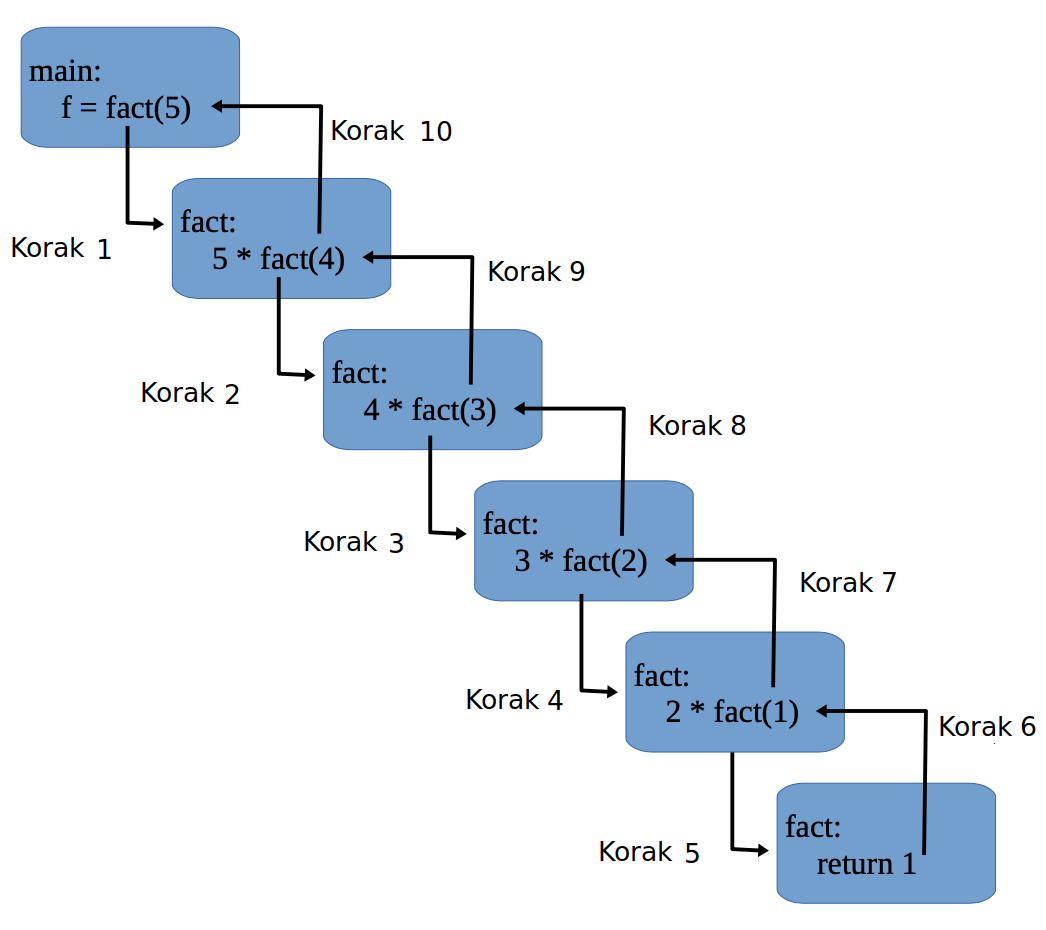
\includegraphics[width=220pt,height=160pt]{slike/factorial_recursion_tree.png}
	\caption{Drvo rekurzivnih poziva za funkciju faktorijela.}
	\label{fig:rec_tree}
\end{figure}

\textbf{Vremenska složenost.}
Broj rekurzivnih poziva proporcionalan je vrijednosti parametra $n$, pa je složenost $ O(n).$

\subsection{Prekoračenje steka}

Ako bazni slučaj nije pravilno definisan ili nije dostižan, rekurzija se neće završiti. Posmatrajmo sljedeći primjer:

\begin{minted}{python}
	def fact(n):
	
	    if n == 100:
	        return 1
	    return n * fact(n - 1)
\end{minted}

Ukoliko je početna vrijednost parametra manja od 100, funkcija će nastaviti da poziva samu sebe sa sve manjim vrijednostima argumenta i nikada neće dostići bazni slučaj. Posljedica je prekoračenje maksimalne dubine rekurzije i aktiviranje izuzetka:

\begin{minted}{python}
	RecursionError:
	maximum recursion depth exceeded
\end{minted}

Maksimalna dozvoljena dubina rekurzije može se provjeriti i po potrebi izmijeniti pomoću funkcija modula \texttt{sys}, iako se povećanje ove granice uglavnom ne preporučuje.

\section{Vrste rekurzije}

Rekurzivne funkcije mogu se klasifikovati na više načina.

\subsection*{Direktna i indirektna rekurzija}

Funkcija je \textit{direktno rekurzivna} ukoliko poziva samu sebe. Funkcija je \textit{indirektno rekurzivna} ukoliko poziva drugu funkciju koja, direktno ili indirektno, ponovo poziva prvu funkciju.

\begin{minted}{python}
	
	# Direktna rekurzija
	
	def direktna():
	    direktna()
	
	# Indirektna rekurzija
	def funkcija1():
	     funkcija2()
	
	def funkcija2():
	    funkcija1()
\end{minted}

\subsection*{Repna i nerepna rekurzija}

Rekurzija se naziva \textit{repnom} (eng. \textit{tail recursion}) ukoliko je rekurzivni poziv posljednja operacija koja se izvršava u funkciji.

\begin{minted}{python}
	def countdown(n):
	
	    if n == 0:
	        return
	    return countdown(n - 1)
	
\end{minted}

U suprotnom govorimo o \textit{nerepnoj rekurziji}. Na primjer:

\begin{minted}{python}
	def fact(n):
	
	    if n == 0:
	        return 1
	
	    return n * fact(n - 1)
	
\end{minted}

Pošto se nakon povratka iz rekurzivnog poziva još uvijek izvršava operacija množenja, funkcija \texttt{fact()} predstavlja primjer nerepne rekurzije.

Iako neki programski jezici optimizuju repnu rekurziju, standardna implementacija Pajtona (CPython) ne primjenjuje ovu optimizaciju. Zbog toga duboke rekurzije mogu dovesti do povećane potrošnje memorije i pojave izuzetka \texttt{RecursionError}.

 
\subsection{Rekurzivni i iterativni pristup: poređenje}

Svaki rekurzivni algoritam može se implementirati i u iterativnom obliku, korištenjem petlji i odgovarajućih pomoćnih struktura podataka. Iako oba pristupa imaju istu računarsku moć, među njima postoje značajne razlike.

\begin{itemize}
	\item Rekurzija se završava dostizanjem baznog slučaja, dok se iteracija završava kada uslov petlje postane netačan.
	
	\item Rekurzija je zasnovana na pozivima funkcija, dok se iteracija zasniva na petljama (\texttt{for} i \texttt{while}).
	
	\item Svaki rekurzivni poziv zauzima dodatni prostor u memoriji steka, dok iterativni algoritmi uglavnom zahtijevaju manje dodatne memorije.
	
	\item Rekurzivna rješenja često su kraća i bliža matematičkoj formulaciji problema, dok iterativna rješenja mogu biti nešto duža što se tiče k\^oda, ali su obično efikasnija.	
\end{itemize}

Rekurzivni programi najčešće zahtijevaju više memorije od ekvivalentnih iterativnih programa, jer se informacije o svakom pozivu funkcije čuvaju u steku sve do dostizanja baznog slučaja. Takođe, dodatno vrijeme izvršavanja troši se na pozivanje funkcija i povratak rezultata.

S druge strane, rekurzija često omogućava elegantnije i preglednije implementacije. Neki problemi prirodno imaju rekurzivnu strukturu, kao što su obilazak stabala, problem Hanojskih kula, generisanje kombinacija i permutacija, te različiti algoritmi zasnovani na paradigmi \emph{podijeli pa zavladaj}. U takvim situacijama rekurzivni pristup često predstavlja intuitivnije rješenje.

\subsection{Primjene rekurzije}

Rekurzija se koristi u brojnim oblastima informatike i programiranja. %Neke od najvažnijih primjena su:

\begin{enumerate}
	
	\item \textbf{Pretraga stabala i grafova}: Rekurzija se prirodno koristi za obilazak hijerarhijskih struktura podataka kao što su stabla i grafovi. Primjeri su algoritmi DFS (eng. \emph{Depth-First Search}) i različiti obilaci binarnih stabala.
	
	\item \textbf{Algoritmi sortiranja}: Mnogi poznati algoritmi sortiranja koriste rekurziju. Primjeri su Brzo sortiranje i Sort spajanjem, koji problem sortiranja razlažu na manje podprobleme i zatim kombinuju njihova rješenja.
	
	\item \textbf{Generisanje fraktala}:  Brojni fraktalni objekti mogu se generisati primjenom rekurzivnih pravila. Jedan od najpoznatijih primjera je Mandelbrotov skup.
	
	\begin{figure}[H]
		\centering
		
\includegraphics[width=100pt,height=80pt]{slike/mandelbrot.png}
		\caption{Mandelbrotov skup.}
	\end{figure}
	
	\item \textbf{Algoritmi vraćanja unazad}:  Ovi algoritmi postepeno grade rješenje problema. Kada se ustanovi da trenutno parcijalno rješenje ne može dovesti do validnog konačnog rješenja, algoritam se vraća na prethodno stanje i pokušava drugu mogućnost.
	
	\item \textbf{Dinamičko programiranje i memoizacija}:	Memoizacija predstavlja tehniku pohranjivanja prethodno izračunatih rezultata podproblema kako bi se izbjeglo njihovo ponovno računanje. Ova tehnika se često koristi zajedno sa rekurzijom i predstavlja osnovu mnogih algoritama dinamičkog programiranja.
\end{enumerate}

U nastavku ćemo ilustrovati primjenu rekurzije na nekoliko konkretnih problema.

\begin{example}
	Pretpostavimo da se populacija zečeva razvija prema sljedećem pravilu. Par zečeva tokom prvog mjeseca života ne daje potomstvo. Počevši od drugog mjeseca života, svaki par na kraju svakog mjeseca proizvede jedan novi par zečeva. Koliko će novih parova zečeva biti nakon 12 mjeseci?
\end{example}

\begin{solution}
	
	Broj novorođenih parova po mjesecima formira niz $$[0,1,1,2,3,5,8,13,21,\ldots].$$
	
	Poznat je kao Fibonačijev niz. Ako sa $f(n)$ označimo broj novorođenih parova na kraju $n$-tog mjeseca, tada važi rekurzivna relacija
	$ f(n)=f(n-1)+f(n-2), n\geq 2,$ uz bazne slučajeve $f(0)=0, f(1)=1. $
	
\end{solution}

Odgovarajuća rekurzivna implementacija glasi:

\begin{minted}{python}
	def fib(n):
	    if n == 0:
	        return 0
	
	    if n == 1:
	        return 1
	
	    return fib(n - 1) + fib(n - 2)
\end{minted}

U svakom netrivijalnom koraku funkcija generiše dva nova rekurzivna poziva. Zbog toga se broj poziva vrlo brzo povećava sa rastom vrijednosti parametra $n$.

\textbf{Vremenska složenost.}  Za funkciju vrijedi rekurentna relacija $T(n)=T(n-1)+T(n-2)+O(1).$

Rješenje ove rekurencije ima eksponencijalni rast, pa je vremenska složenost $
T(n)=O(\varphi^n),$ gdje je $\varphi=\frac{1+\sqrt{5}}{2}\approx 1.618$ zlatni presjek. U literaturi se često koristi i grublja ocjena $ T(n)=O(2^n).$

Ovaj primjer pokazuje da rekurzija sama po sebi ne garantuje efikasan algoritam. U narednim poglavljima vidjećemo kako se primjenom memoizacije i dinamičkog programiranja složenost računanja Fibonačijevih brojeva može smanjiti sa eksponencijalne na linearnu.


%fib_rec.jpeg
\begin{figure}[H]
	\centering
	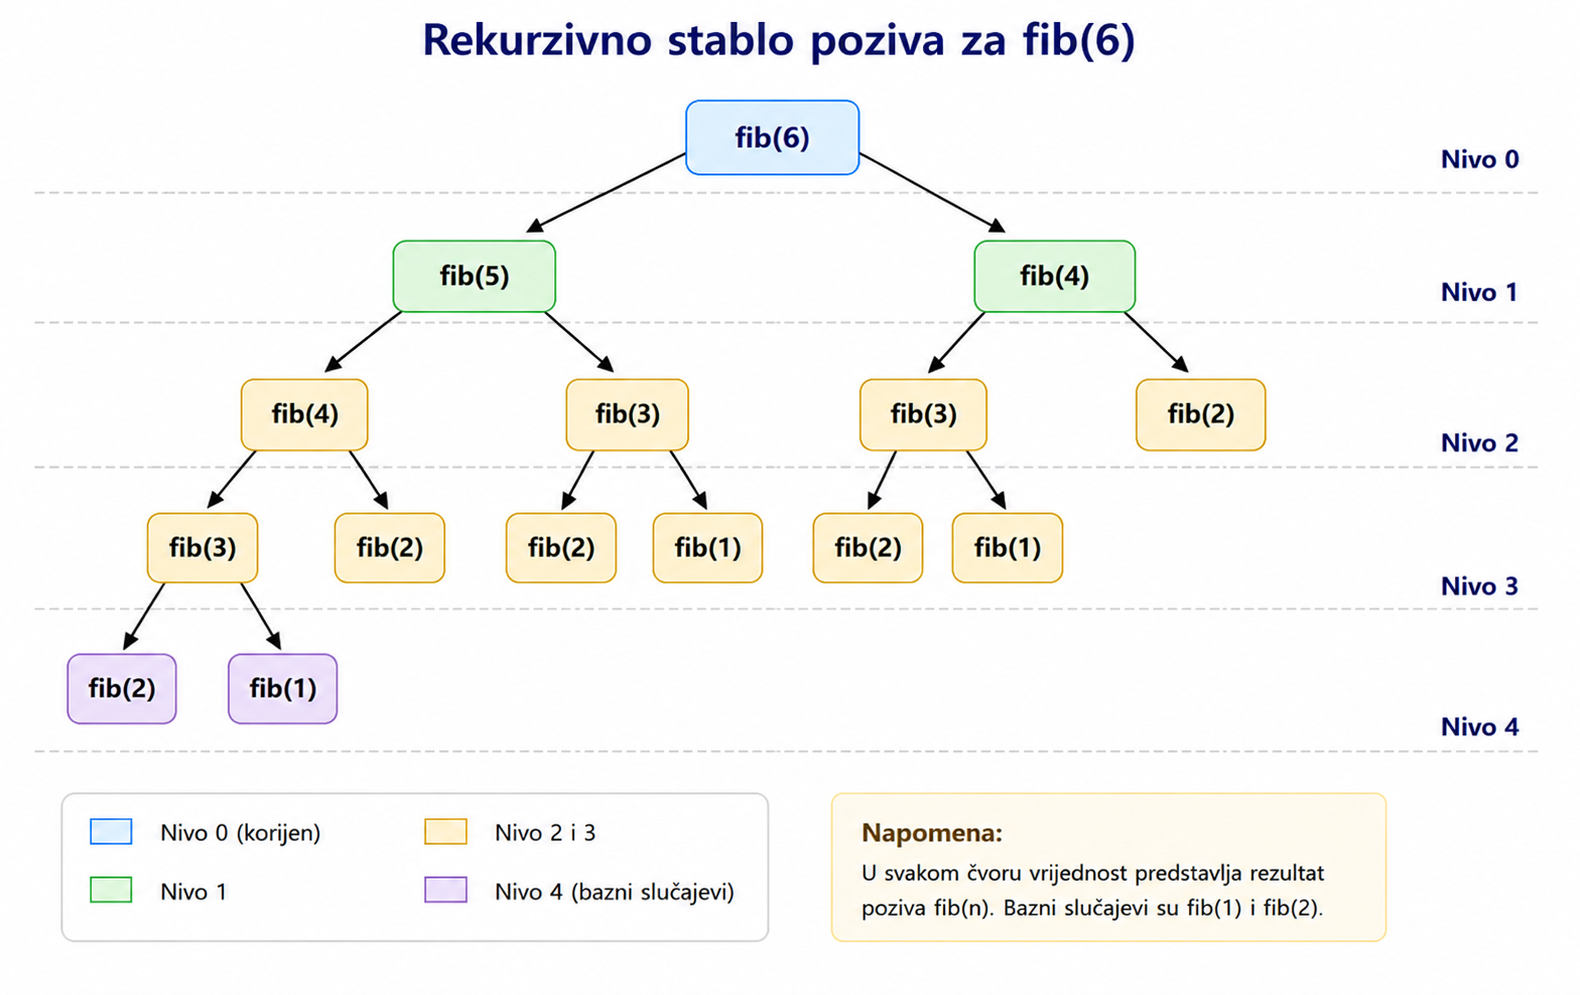
\includegraphics[width=250pt,height=140pt]{slike/fib_rec.png} 
	\label{fig:rec_fib}
	\caption{Drvo rekurzije za \texttt{fib} rekurzivni metod.}
\end{figure}


\begin{example}
	\textbf{(\emph{Problem Hanojskih kula})}
	
	Data su tri štapa i $n$ diskova različitih dimenzija. Svi diskovi su inicijalno složeni na jednom štapu ($A$), pri čemu se manji diskovi nalaze iznad većih. Cilj je premjestiti kompletnu kulu diskova na drugi štap ($C$), koristeći treći štap ($B$) kao pomoćni.
	
	Pri tome moraju biti zadovoljena sljedeća pravila:
	
	\begin{itemize}
		\item U jednom potezu dozvoljeno je premjestiti samo jedan disk.
		
		\item Disk se uvijek uzima sa vrha jednog štapa i postavlja na vrh drugog štapa.
		
		\item Veći disk nikada ne smije biti postavljen na manji disk.
		
	\end{itemize}
	
	Odrediti minimalan broj poteza potreban za premještanje svih diskova sa štapa $A$ na štap $C$.
\end{example}

\begin{solution}
	
	Najprije razmotrimo slučaj sa dva diska ($n=2$). Pretpostavimo da se oba diska nalaze na štapu $A$, a da ih želimo premjestiti na štap $C$.
	
	Rješenje se sastoji od tri poteza:
	
	\begin{enumerate}
		\item manji disk se premješta sa štapa $A$ na štap $B$;
		\item veći disk se premješta sa štapa $A$ na štap $C$;
		\item manji disk se premješta sa štapa $B$ na štap $C$.
	\end{enumerate}
	
	Posmatrajmo sada slučaj sa tri diska ($n=3$), prikazan na Slici~\ref{fig:tower}.
	
	\begin{figure}[H]
		\centering
		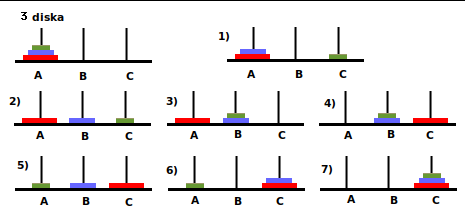
\includegraphics[width=270pt,height=150pt]{slike/tower.png}
		\caption{Problem Hanojskih kula za $n=3$ diska.}
		\label{fig:tower}
	\end{figure}
	
	Rješenje se dobija sljedećim redoslijedom poteza:
	
	\begin{enumerate}
		\item najmanji disk se premješta sa štapa $A$ na štap $C$;
		\item srednji disk se premješta sa štapa $A$ na štap $B$;
		\item najmanji disk se premješta sa štapa $C$ na štap $B$;
		\item najveći disk se premješta sa štapa $A$ na štap $C$;
		\item najmanji disk se premješta sa štapa $B$ na štap $A$;
		\item srednji disk se premješta sa štapa $B$ na štap $C$;
		\item najmanji disk se premješta sa štapa $A$ na štap $C$.
	\end{enumerate}
	
	Ukupno je potrebno sedam poteza.\\
	
	Da bismo riješili opšti slučaj, označimo sa $T(n)$ minimalan broj poteza potreban za premještanje $n$ diskova sa štapa $A$ na štap $C$, koristeći štap $B$ kao pomoćni.
	
	Bazni slučaj je jednostavan: $	T(1)=1.$  Za proizvoljno $n>1$, najprije je potrebno premjestiti gornjih $n-1$ diskova sa štapa $A$ na štap $B$, koristeći štap $C$. Za to je potrebno $T(n-1)$ poteza.  Nakon toga najveći disk ostaje sam na štapu $A$ i može se direktno premjestiti na štap $C$ u jednom potezu.
	
	Preostaje da se $n-1$ diskova sa štapa $B$ rekurzivno premjesti na štap $C$, za šta je ponovo potrebno $T(n-1)$ poteza.  	Prema tome, ukupan broj poteza zadovoljava rekurentnu relaciju $ T(n)=T(n-1)+1+T(n-1),$  odnosno	$	T(n)=2T(n-1)+1, 	T(1)=1.$ Prethodni postupak opisuje rekurzivnu formulaciju problema Hanojskih kula.
	
	Rješavanjem navedene rekurencije dobija se zatvorena forma $T(n)=2^n-1.$	Dakle, minimalan broj poteza potreban za premještanje $n$ diskova iznosi 	$2^n-1.$ Na primjer, za $n=3$ dobijamo $T(3)=2^3-1=7,$ što se slaže sa prethodno izvedenim rješenjem.
\end{solution}

Implementacija rekurzivnog pristupa problema Hanojskih kula je data sljedećim k\^odom. 

\begin{minted}{python}
	 
	def TowerOfHanoi(n , izvor, cilj, pomocni):
	    if n==1:
	        print ("Pomaknite disk 1 sa štapa ", izvor," \ 
	        na štap ", cilj)
	        return
	    TowerOfHanoi(n-1, izvor, pomocni, cilj)
	    print ("Pomakni disk ",n," sa štapa ", izvor," na štap  \ 
	     ", cilj) #pomijeranje najvećeg štapa
	    TowerOfHanoi(n-1, pomocni, cilj, izvor)
	
	#instanca:
	n = 4 #broj diskova
	TowerOfHanoi(n, 'A','C','B')
\end{minted} 

\textbf{Vremenska kompleksnost}. Vrlo lako dobijamo eksplicitnu funkciju koja odgovara   rekurzivnoj relaciji problema: $T(n)= 2  T(n-1) + 1 = 2 \cdot ( 2 \cdot T(n-2) + 1) + 1 = \cdots = 2^{n-2} + 2^{n-1} + \cdots + 2 + 1 = 2^n -1.$
Rekurzija se izvrašava u eksponencijalnom $O(2^n)$ vremenu.   
\end{solution}	
 

\begin{example}
  
     Sortiranje umetanjem (\emph{Insertion Sort}) predstavlja jednostavan algoritam
     sortiranja koji niz gradi postepeno, održavajući   jedan njegov dio sortiranim. Ideja algoritma sastoji se u tome da se  svaki novi element umetne na odgovarajuću poziciju unutar već sortiranog dijela niza. Niz koji se sastoji od jednog elementa se smatra sortiranim. 
 \end{example}
 
\begin{solution}
    Algoritam sortiranja umetanjem može se prirodno formulirati i rekurzivno.
     Neka je dat niz
 \[
 A = (a_0,a_1,\ldots,a_{n-1})
 \]
 od $n$ elemenata koje je potrebno sortirati u neopadajućem poretku.
 
 Rekurzivna formulacija zasniva se na sljedećem zapažanju. Pretpostavimo da smo
 već sortirali prvih $n-1$ elemenata niza:
 \[
 (a_0,a_1,\ldots,a_{n-2}).
 \]
 Tada je za sortiranje kompletnog niza dovoljno posljednji element
 $a_{n-1}$ umetnuti na odgovarajuću poziciju unutar već sortiranog prefiksa.
 
 Prema tome, algoritam se sastoji od dvije osnovne faze:
 
 \begin{enumerate}
 	\item rekurzivno sortirati prvih $n-1$ elemenata niza;
 	\item umetnuti posljednji element $a_{n-1}$ na odgovarajuću poziciju
 	unutar sortiranog prefiksa.
 \end{enumerate}
 
 Bazni slučaj nastupa kada niz sadrži najviše jedan element. Takav niz je već
 sortiran, pa nije potrebno izvršavati dodatne operacije.
 
 Pretpostavimo sada da su elementi
 \[
 a_0,a_1,\ldots,a_{n-2}
 \]
 već sortirani. Vrijednost $a_{n-1}$ privremeno čuvamo u promjenljivoj
 \texttt{key}. Zatim se, počevši od elementa $a_{n-2}$, krećemo unazad kroz
 sortirani dio niza. Svaki element koji je veći od vrijednosti \texttt{key}
 pomjera se za jednu poziciju udesno. Kada pronađemo prvi element koji nije
 veći od \texttt{key}, vrijednost \texttt{key} umećemo neposredno iza njega.
 
 Na ovaj način nakon završetka postupka prvih $n$ elemenata niza nalazi se u sortiranom poretku.
\end{solution}
% Pseudokod rekurzivnog algoritma dat je Algoritmom~\ref{alg:recursive-insertion-sort}.
 
%PSEUDOKOD:
\begin{minted}[fontsize=\footnotesize]{python}
	def RecursiveInsertionSort(A, n):
	    if n <= 1:
	        return
	
	    # Rekurzivno sortiramo prvih n-1 elemenata
    	RecursiveInsertionSort(A, n - 1)
	
	    # Umetanje posljednjeg elementa
	    key = A[n - 1]
	    j = n - 2
	
	    while j >= 0 and A[j] > key:
	        A[j + 1] = A[j]
	        j = j - 1
	
	    A[j + 1] = key
\end{minted}


 
 Na primjer, posmatrajmo niz
 \[
 A=[7,3,5,2].
 \]
 Rekurzivni algoritam najprije sortira prefiks dužine $3$,
 odnosno niz $
 [7,3,5],$
 koji nakon sortiranja postaje $
 [3,5,7].$ 
 Preostaje umetanje posljednjeg elementa $2$. Pošto je $2$ manje od svih
 elemenata sortiranog prefiksa, elementi $7$, $5$ i $3$ pomjeraju se za jednu
 poziciju udesno, nakon čega se vrijednost $2$ postavlja na početak niza.
 Dobijamo konačno sortirani niz $
 [2,3,5,7].$
 
 \paragraph{Ispravnost algoritma.} Ispravnost rekurzivnog algoritma možemo pokazati indukcijom po veličini
 niza $n$. Za $n=1$ niz sadrži samo jedan element i trivijalno je sortiran.  Pretpostavimo sada da algoritam ispravno sortira svaki niz od $n-1$
 elemenata. Pri pozivu algoritma za niz od $n$ elemenata, rekurzivni poziv
 sortira njegovih prvih $n-1$ elemenata. Nakon toga posljednji element
 $a_{n-1}$ umeće se na odgovarajuću poziciju unutar sortiranog prefiksa,
 pri čemu se svi elementi veći od njega pomjeraju za jednu poziciju udesno.
 Prema tome, nakon umetanja svih $n$ elemenata nalazi se u neopadajućem
 poretku. Time je pokazano da algoritam ispravno sortira niz proizvoljne
 dužine $n$.
 
 \paragraph{Vremenska složenost.}
 Neka je $T(n)$ vrijeme potrebno za sortiranje niza od $n$ elemenata.
 
 Algoritam najprije rekurzivno sortira prvih $n-1$ elemenata, što zahtijeva
 vrijeme $T(n-1)$. Nakon toga posljednji element umeće se u već sortirani
 prefiks.
 
 U najgorem slučaju posljednji element je manji od svih prethodnih elemenata.
 Tada je potrebno pomjeriti svih $n-1$ elemenata za jednu poziciju udesno.
 Zbog toga operacija umetanja zahtijeva $\Theta(n)$ vremena.
 
 Dobijamo rekurentnu relaciju
 \[
 T(n)=T(n-1)+\Theta(n),
 \]
 uz bazni slučaj
 \[
 T(1)=\Theta(1).
 \]
 
 Razvijanjem rekurzije dobijamo
 \[
 \begin{aligned}
 	T(n)
 	&= T(n-1)+\Theta(n)\\
 	&= T(n-2)+\Theta(n-1)+\Theta(n)\\
 	&\;\;\vdots\\
 	&= T(1)+\Theta(2)+\Theta(3)+\cdots+\Theta(n).
 \end{aligned}
 \]
 
 Kako vrijedi
 \[
 1+2+\cdots+n=\frac{n(n+1)}{2},
 \]
 slijedi
 \[
 T(n)=\Theta(n^2).
 \]
 
 Prema tome, vremenska složenost rekurzivnog algoritma sortiranja umetanjem
 u najgorem slučaju iznosi ${\Theta(n^2)}.$
 
 Najgori slučaj nastupa kada je početni niz sortiran u opadajućem poretku.
 Tada se pri svakom umetanju trenutni element mora pomjeriti preko svih
 prethodno obrađenih elemenata.
 
 U najboljem slučaju niz je već sortiran. Tada se pri svakom rekurzivnom
 nivou izvršava samo jedno poređenje prije nego što se utvrdi da se
 posljednji element već nalazi na odgovarajućoj poziciji. Rekurentna relacija
 tada ima oblik
 \[
 T_{\mathrm{best}}(n)
 =
 T_{\mathrm{best}}(n-1)+\Theta(1),
 \]
 odakle slijedi
 \[
 T_{\mathrm{best}}(n)=\Theta(n).
 \]
 
 Prosječna vremenska složenost algoritma iznosi $
 \Theta(n^2).$
 
 \paragraph{Prostorna složenost.}
 Sama operacija umetanja koristi samo konstantan broj dodatnih promjenljivih.
 Međutim, zbog rekurzivne implementacije na steku se istovremeno može nalaziti
 do $n$ aktivnih poziva funkcije. Zbog toga dodatna prostorna složenost
 rekurzivnog algoritma iznosi $\Theta(n)$.
 
 Kod standardne iterativne implementacije sortiranja umetanjem ovaj dodatni
 trošak ne postoji, pa je njena prostorna složenost $\Theta(1)$.
 
 Sortiranje umetanjem nije efikasno za velike nizove zbog kvadratne prosječne
 i najgore vremenske složenosti. Ipak, algoritam ima nekoliko važnih
 prednosti. Jednostavan je za implementaciju, ne zahtijeva dodatnu memoriju
 za čuvanje elemenata i veoma je efikasan za male ili skoro sortirane nizove.
 
 Rekurzivna formulacija posebno je korisna sa pedagoškog stanovišta, jer
 jasno pokazuje način na koji se problem veličine $n$ može svesti na problem
 istog tipa veličine $n-1$. Time sortiranje umetanjem predstavlja jednostavan
 primjer primjene rekurzivnog načina razmišljanja na problem sortiranja.

\section{Algoritmi grube sile}

Algoritmi grube sile predstavljaju jednu od najjednostavnijih algoritamskih paradigmi za rješavanje računarskih problema. Osnovna ideja ove paradigme jeste sistematsko ispitivanje svih mogućih rješenja dok se ne pronađe rješenje koje zadovoljava postavljene uslove ili dok se ne odredi najbolje rješenje prema zadanom kriterijumu.

Iako je riječ o jednostavnom pristupu, algoritmi grube sile imaju značajnu ulogu u algoritamskom dizajnu. Često predstavljaju polaznu tačku za razvoj efikasnijih algoritama, a za probleme manjih dimenzija mogu dati zadovoljavajuća rješenja.

U svakodnevnom životu primjer algoritma grube sile je pokušaj otključavanja brave kada ne znamo koji ključ odgovara. U tom slučaju isprobavamo jedan po jedan ključ sve dok ne pronađemo odgovarajući. Slično tome, ukoliko ne znamo orijentaciju USB priključka, pokušavamo jednu mogućnost, a zatim drugu.

Paradigma grube sile može se koristi za:

\begin{itemize}
	\item probleme pretraživanja,
	\item probleme zadovoljenja ograničenja (SAT problemi),
	\item probleme optimizacije,
	\item verifikaciju ispravnosti složenijih algoritama.
\end{itemize}

\begin{example}(\textbf{Problem najbližeg para tačaka}) Neka je dat skup od $n$ tačaka u prostoru $\mathbb{R}^m$:
	
	\[
	S=\{\mathbf{x}_1,\mathbf{x}_2,\ldots,\mathbf{x}_n\}.
	\]
	
	Potrebno je pronaći dvije tačke iz skupa $S$ čija je međusobna Euklidova udaljenost najmanja.
	
\end{example}

\begin{solution}
	
	Pristup grube sile podrazumijeva izračunavanje udaljenosti između svakog para tačaka iz skupa $S$. Tokom izvršavanja algoritma pamtimo najmanju do sada pronađenu udaljenost i odgovarajući par tačaka.
	
	Jedna moguća implementacija prikazana je u nastavku.
	
	\begin{minted}{python}
		import math
		
		def min_dist_pair(S):
		
		    min_dist = float("inf")
		    point1 = None
		    point2 = None
		
		    for i in range(len(S)):
		        for j in range(i + 1, len(S)):
		            distance = math.dist(S[i], S[j])
		
		            if distance < min_dist:
		                min_dist = distance
		                point1 = S[i]
		                point2 = S[j]
		
		    return point1, point2, min_dist
		
	\end{minted}
	
\end{solution}

\textbf{Analiza složenosti.} Broj različitih parova tačaka jednak je $\binom{n}{2}=\frac{n(n-1)}{2}=O(n^2).$  Računanje Euklidove udaljenosti između dvije tačke u prostoru $\mathbb{R}^m$ se vrši u $O(m)$ vremenu. Kako je dimenzija prostora $m$ fiksna, ukupna vremenska složenost algoritma iznosi $O(n^2).$

\vspace{0.3cm}

\begin{example}
	(\textbf{Problem ruksaka}). 
	Neka je dato $n$ predmeta. Svaki predmet $i$ ima težinu $w_i$ i vrijednost $p_i$, za svaki $i=1,\ldots,n$. Takođe je dat ruksak kapaciteta $C$.\\
	Potrebno je odabrati predmete koje treba staviti u ruksak tako da njihova ukupna težina ne prelazi kapacitet ruksaka, a pri tome je ukupna vrijednost u ruksaku najveća moguća.

\end{example}

\begin{solution}
	
	Posmatrajmo sljedeću instancu problema.
	
	\begin{center}
		\begin{tabular}{ccc}
			\emph{Predmet} & \emph{Težina} & \emph{Vrijednost} \\ \hline
			1 & 2  & 20 \\
			2 & 5  & 30 \\
			3 & 10 & 50 \\
			4 & 5  & 10 \\ \hline \hline
		\end{tabular}
	\end{center}
	
	Neka je kapacitet ruksaka $C=16.$	Pristup grube sile sastoji se u generisanju svih mogućih podskupova skupa predmeta. Kako postoje četiri predmeta, ukupan broj mogućih rješenja jednak je $2^4 = 16.$
	
	Za svaki podskup izračunava se ukupna težina i ukupna vrijednost.
	
	\begin{center}
		\begin{tabular}{lcc}
			Rješenje & Ukupna težina & Ukupna vrijednost \\ \hline
			$\{1\}$ & 2 & 20  \\
			$\{2\}$ & 5 & 30  \\
			$\{3\}$ & 10 & 50  \\
			$\{4\}$ & 5 & 10  \\
			$\{1,2\}$ & 7 & 50  \\
			$\{1,3\}$ & 12 & 70  \\
			$\{1,4\}$ & 7 & 30  \\
			$\{2,3\}$ & 15 & 80  \\
			$\{2,4\}$ & 10 & 40  \\
			$\{3,4\}$ & 15 & 60 \\
			$\{1,2,3\}$ & 17 & nedopustivo  \\
			$\{1,2,4\}$ & 12 & 60  \\
			$\{1,3,4\}$ & 17 & nedopustivo  \\
			$\{2,3,4\}$ & 20 & nedopustivo  \\
			$\{1,2,3,4\}$ & 22 & nedopustivo  \\ \hline
		\end{tabular}
	\end{center}
	
	Iz tabele se vidi da optimalno rješenje odgovara skupu $\{2,3\},$ čija je ukupna težina $15$, a ukupna pridružena vrijednost $80$.
	
\end{solution}

Pošto se svaki predmet može ili nalaziti ili ne nalaziti u ruksaku, prostor rješenja odgovara skupu svih podskupova skupa $\{1,\ldots,n\}$. Broj mogućih rješenja jednak je $2^n.$

Zbog toga je vremenska složenost algoritma grube sile eksponencijalna, $O(2^n).$\\

Jedna moguća implementacija prikazana je u nastavku.

\begin{minted}[fontsize=\footnotesize]{python}
	best_fitness = 0
	
	# primjer instance
	N = 4
	w = [2, 5, 10, 5]
	p = [20, 30, 50, 10]
	C = 16
	
	def objective(solution):
	
 	    weight = 0
	    value = 0
	
	    for i in solution:
	        weight += w[i]
	        value += p[i]
	
	    if weight > C:
	        return float("-inf")
	    return value
	
	def knapsack_brute_force(solution):
	
	
	    global best_fitness
	    
	    best_fitness = max(
	        best_fitness,
	        objective(solution))
	
	    for i in range(N):
	
	        if len(solution) == 0:
	            knapsack_brute_force([i])
	
	        elif i > max(solution): #razbijanje simetrije
	            knapsack_brute_force(solution + [i])
	
	knapsack_brute_force([])
	print(best_fitness)   # 80
\end{minted}

Algoritmi grube sile obično nisu praktični za velike instance problema zbog eksponencijalnog ili polinomijalno visokog vremena izvršavanja. Ipak, oni imaju značajnu teorijsku vrijednost jer garantuju pronalaženje optimalnog rješenja i često predstavljaju osnovu za razvoj efikasnijih algoritama zasnovanih na paradigmi \emph{podijeli pa zavladaj}, dinamičkom programiranju, grananju i ograničavanju (eng. \emph{branch-and-bound}) ili metaheuristikama.


Kako primjećujemo na osnovu prethodne (rekurzivne) implementacije, svaki od  
rekurzivnih poziva, kojih je tačno $2^n$, poziva funkciju \texttt{objective}. Preciznije, kompleksnost pristupa brutalne sile je $O(2^n)$. Napomenimo da postoje efikasniji pristupi za rješavanje problema ruksaka. Među njima, izdvajamo metod dinamičkog programiranja, o kojem će biti više riječi u nastavku.


\section{Algoritmi pretraživanja}

Algoritmi pretraživanja predstavljaju grupu algoritama čiji je zadatak pronalaženje određenog elementa unutar strukture podataka. Rezultat pretrage najčešće je informacija da li traženi element postoji, a ukoliko postoji, vraća se njegova pozicija ili druga relevantna informacija o njemu.

Algoritmi pretraživanja imaju široku primjenu u računarstvu, od rada sa nizovima i listama do pretraživanja baza podataka, tekstualnih dokumenata i složenih struktura podataka.

U zavisnosti od načina organizacije podataka i strategije pretraživanja, algoritmi pretraživanja mogu se podijeliti u dvije osnovne kategorije:

\begin{itemize}
	\item \textit{Sekvencijalna pretraga} prolazi kroz elemente strukture jedan po jedan sve dok ne pronađe traženi element ili ne iscrpi cijelu strukturu. Najpoznatiji predstavnik ove grupe je \textit{linearna pretraga}.
	
	\item \textit{Intervalna pretraga} koristi dodatne informacije o organizaciji podataka, najčešće činjenicu da su podaci sortirani. Umjesto provjeravanja svih elemenata, prostor pretrage se postepeno smanjuje, čime se postiže znatno veća efikasnost. Najpoznatiji primjer je \textit{binarna pretraga}.

\end{itemize}

\subsection{Linearna pretraga}

Linearna pretraga (eng. \emph{linear search}) predstavlja najjednostavniji algoritam pretraživanja. Ideja algoritma je da se elementi strukture podataka obilaze redom, od početka prema kraju, sve dok se ne pronađe tražena vrijednost.

U slučaju da se traženi element pronađe, algoritam vraća njegov indeks. Ukoliko se dođe do kraja strukture bez pronalaska elementa, vraća se posebna vrijednost koja označava neuspješnu pretragu.

Iterativna implementacija linearne pretrage prikazana je u nastavku.

\begin{minted}{python}
	def search(arr, x):
	
	
	    for i in range(len(arr)):
	        if arr[i] == x:
	        return i
	
	    return -1
	
	arr = [2, 3, 1, 11, 10, 20]
	x = 10
	res = search(arr, x)
	
	if res == -1:
	    print("Element nije pronađen.")
	else:
	    print("Element je pronađen na indeksu", res)
\end{minted}

\textbf{Analiza složenosti.} U najgorem slučaju algoritam mora pregledati svih $n$ elemenata strukture podataka. Zbog toga je vremenska složenost linearne pretrage $O(n),$  gdje je $n$ broj elemenata u strukturi. Dodatna memorija koja se koristi tokom izvršavanja algoritma je konstantna, pa je prostorna složenost jednaka $O(1).$

\vspace{0.3cm}

Linearna pretraga može se implementirati i rekurzivno.

\begin{minted}{python}
	def linear_search(arr, x, i):
	
	    if i >= len(arr):
	        return -1
	    if arr[i] == x:
	        return i
	
	    return linear_search(arr, x, i + 1)
	
	# poziv funkcije
	res = linear_search(arr, x, 0)
\end{minted}

Kod rekurzivne implementacije vremenska složenost ostaje nepromijenjena i iznosi $O(n)$. Međutim, svaki rekurzivni poziv zauzima dodatni prostor na steku, pa je prostorna složenost $O(n).$

\textit{Prednosti i nedostaci.}  Glavna prednost linearne pretrage jeste njena jednostavnost. Algoritam ne zahtijeva nikakvu prethodnu obradu podataka niti sortiranje strukture nad kojom se vrši pretraga. Zbog toga se može primijeniti na bilo kojem nizu, listi ili drugoj sekvencijalnoj strukturi podataka.

Sa druge strane, linearna pretraga nije efikasna za velike skupove podataka, jer se broj potrebnih poređenja povećava proporcionalno veličini ulaza. Iz tog razloga koristi se uglavnom za manje strukture podataka ili u situacijama kada podaci nisu sortirani i kada jednostavnost implementacije ima prednost nad efikasnošću izvršavanja.

\subsection{Binarna pretraga}

Binarna pretraga (eng. \emph{binary search}) predstavlja jedan od najefikasnijih algoritama za pretraživanje podataka. Za razliku od linearne pretrage, koja elemente provjerava redom, binarna pretraga u svakoj iteraciji eliminiše približno polovinu preostalog prostora pretrage.

Da bi se binarna pretraga mogla primijeniti, moraju biti zadovoljena dva osnovna uslova:

\begin{enumerate}
	\item podaci moraju biti sortirani;
	\item pristup proizvoljnom elementu strukture mora biti moguć u konstantnom vremenu.
\end{enumerate}

Pretpostavimo da je niz sortiran u rastućem poretku. U svakoj iteraciji određuje se srednji element trenutnog intervala pretrage i poredi sa traženom vrijednošću $x$.

Moguća su tri slučaja:

\begin{itemize}
	\item ako je srednji element jednak vrijednosti $x$, pretraga se završava;
	\item ako je srednji element veći od $x$, traženi element se može nalaziti samo u lijevoj polovini niza;
	\item ako je srednji element manji od $x$, pretraga se nastavlja u desnoj polovini niza.
\end{itemize}

Na taj način se u svakom koraku prostor pretrage prepolovljava.

Rekurzivna implementacija binarne pretrage prikazana je u nastavku.

\begin{minted}{python}
	def binary_search(arr, x):

	    if len(arr) == 0:
	        return False
	
	    if len(arr) == 1:
	        return arr[0] == x
	    mid = len(arr) // 2
	
	    if arr[mid] == x:
	        return True
	    elif arr[mid] < x:
	        return binary_search(arr[mid + 1:], x)
	    else:
	        return binary_search(arr[:mid], x)
	
	# primjer poziva
	
	arr = [2, 8, 10, 12, 15]
	x = 10
	found = binary_search(arr, x)
	print(found)
\end{minted}

\textbf{Analiza složenosti.} Neka je $T(n)$ vrijeme izvršavanja algoritma za niz dužine $n$. U svakoj iteraciji pretražuje se samo jedna polovina niza, pa vrijedi rekurentna relacija $T(n)=T\left(\frac{n}{2}\right)+O(1).$ Primjenom Master teoreme dobija se $T(n)=O(\log n).$ Dakle, binarna pretraga je značajno efikasnija od linearne pretrage čija je složenost $O(n)$.

Binarna pretraga se posebno koristi kod velikih sortiranih skupova podataka, gdje njena logaritamska složenost omogućava veoma brzo pronalaženje traženih elemenata.

\subsection{Pretraga preskakanjem}

Pretraga preskakanjem (eng. \emph{jump search}) predstavlja kompromis između linearne i binarne pretrage. Kao i binarna pretraga, zahtijeva da podaci budu sortirani.

Osnovna ideja algoritma jeste da se niz ne pretražuje element po element, već da se kroz njega kreće u koracima određene dužine. Na taj način brzo se pronalazi manji interval u kojem se potencijalno nalazi traženi element, nakon čega se unutar tog intervala primjenjuje linearna pretraga.

Pretpostavimo da je dat sortirani niz dužine $n$ i da je veličina koraka jednaka $m$. Algoritam provjerava elemente na pozicijama $0,; m,; 2m,; 3m,\ldots$

sve dok ne pronađe interval koji sadrži traženi element $x$.

Preciznije, traži se prvi indeks $k$ za koji vrijedi $\texttt{niz}[k \cdot m] \geq x.$ Nakon toga vrši se linearna pretraga unutar prethodnog bloka.

Posmatrajmo niz

$$
[0,1,1,2,3,5,8,12,24,37,55,82,140,433,567,622]$$

i pretpostavimo da je potrebno naći vrijednost $x=55$, koristeći korak $m=4.$ Algoritam izvršava sljedeće korake:

\begin{enumerate}
	\item provjerava element na indeksu $0$;
	\item prelazi na indeks $4$;
	\item prelazi na indeks $8$;
	\item prelazi na indeks $12$;
	\item pošto je vrijednost na indeksu $12$ jednaka $140 > 55$, zaključuje da se traženi element nalazi između indeksa $8$ i $12$;
	\item vrši linearnu pretragu unutar tog intervala i pronalazi vrijednost $55$.
\end{enumerate}

\textbf{Analiza složenosti.} U najgorem slučaju potrebno je izvršiti približno $\frac{n}{m}$ skokova, a zatim još najviše $m-1$ poređenja tokom linearne pretrage unutar pronađenog bloka.

Ukupan broj poređenja iznosi $f(m)=\frac{n}{m}+m-1.$
 Minimum ove funkcije postiže se za $m=\sqrt{n}.$ Zamjenom optimalne vrijednosti koraka dobija se vremenska složenost $O(\sqrt{n}).$ Pretraga preskakanjem je sporija od binarne pretrage, ali jednostavnija za implementaciju u pojedinim strukturama podataka kod kojih nije praktično često dijeljenje intervala. Zbog toga predstavlja koristan kompromis između jednostavnosti linearne pretrage i efikasnosti binarne pretrage.

 
 
Rekurzivna implementacija pretage preskakanjem  je data sljedećim k\^odom.  % u jeziku Pajton. 
 
 \begin{minted}[fontsize=\footnotesize]{python}
 def jump_search(niz, x, jump, k):
 
 	if k * jump >= len(niz): #empty array
 		return False
 
 	if k * jump < len(niz) and (k+1) * jump >= len(niz): 
 		found = linear_search(niz[k*jump :], x, 0)
 		return found
 	#rekurzivni korak: oba kraja intervala su elementi niza: 
 	if niz[ k * jump ] <= x and x <= niz[ (k+1) * jump ]:
 		found = linear_search(niz[k*jump: ((k+1)*jump + 1)], x, 0)
 		return found
 	else:
 		return jump_search(niz, x, jump, k+1) # idemo na naredni interval
 
 	#instanca:
 	niz = [2, 10, 21, 33, 38, 41, 45, 52, 57, 70, 75]
 	jump_step = 3
 	x= 57
 	# poziv metoda:
 	found = jump_search(niz, 57, jump_step, 0)
 	print(found) 
 \end{minted}

\subsection{Interpolacijska pretraga}

Interpolacijska pretraga (eng. \emph{interpolation search}) predstavlja unapređenje binarne pretrage namijenjeno radu sa sortiranim nizovima čije su vrijednosti približno ravnomjerno raspoređene. Za razliku od binarne pretrage, koja uvijek ispituje srednji element trenutnog intervala, interpolacijska pretraga pokušava procijeniti poziciju traženog elementa na osnovu njegove vrijednosti.

Osnovna ideja algoritma zasniva se na analogiji sa pretragom riječi u rječniku. Ukoliko tražimo riječ koja počinje slovom „Š“, nećemo otvoriti rječnik na sredini, već bliže njegovom kraju. Slično tome, ako je vrijednost traženog elementa bliža najvećem elementu niza, algoritam će pretragu započeti bliže kraju niza.

Pretpostavimo da je dat sortirani niz $[ niz[0],, niz[1],, \ldots,, niz[n-1] ]$ i da tražimo element vrijednosti $x$. Pozicija na kojoj će se izvršiti naredno poređenje procjenjuje se linearnom interpolacijom između krajnjih elemenata trenutnog intervala pretrage.

Vrijednost indeksa \textit{pos} računa se formulom $
pos=
\left\lfloor
\frac{(n-1),(x-niz[0])}
{niz[n-1]-niz[0]}
\right\rfloor .
$

Drugim riječima, ukoliko je vrijednost $x$ bliža početku intervala, dobiće se manji indeks \textit{pos}; ako je bliža kraju intervala, dobiće se veći indeks.\\

Algoritam se sastoji od sljedećih koraka:

\begin{enumerate}
	\item Izračunati procijenjenu poziciju \textit{pos} koristeći interpolacionu formulu.
	
	\item Ako je $niz[pos] = x$, pretraga se završava i vraća se pronađena pozicija.
	
	\item Ako je $x < niz[pos]$, pretraga se nastavlja u lijevom dijelu niza.
	
	\item Ako je $x > niz[pos]$, pretraga se nastavlja u desnom dijelu niza.
	
	\item Koraci 1--4 ponavljaju se sve dok se element ne pronađe ili dok interval pretrage ne postane prazan.
	
\end{enumerate}

Jedna moguća implementacija interpolacijske pretrage prikazana je u nastavku.

\begin{minted}{python}
	def interpolation_search(arr, x):
	
	    left = 0
	    right = len(arr) - 1
	
	    while (left <= right and x >= arr[left] and \ 
	        x <= arr[right]):
	
	        if left == right:
	            if arr[left] == x:
	                    return left
	                return -1
	
	        pos = left + ((x - arr[left]) * \ 
	              (right - left)) // (arr[right] - arr[left] )
	
	        if arr[pos] == x:
	            return pos
	        elif arr[pos] < x:
	            left = pos + 1
	        else:
	            right = pos - 1
	    return -1
	
\end{minted}

\textbf{Analiza složenosti.} Ako su vrijednosti u nizu približno uniformno raspoređene, interpolacijska pretraga u prosjeku ostvaruje vremensku slože\-nost $O(\log\log n),$ što je bolje od složenosti binarne pretrage, koja iznosi $O(\log n)$.

Međutim, ova prednost postoji samo kada je pretpostavka o približno ravnomjernoj raspodjeli podataka zadovoljena. U nepovoljnom slučaju, kada su podaci izrazito neravnomjerno raspoređeni, vremenska složenost može degradirati na $O(n),$ što odgovara složenosti linearne pretrage. Zbog toga se interpolacijska pretraga koristi prvenstveno kod velikih sortiranih skupova numeričkih podataka za koje se očekuje približno uniformna raspodjela vrijednosti podataka.


\subsection{Eksponencijalna pretraga}

Eksponencijalna pretraga (eng. \emph{exponential search}) predstavlja algoritam pretraživanja namijenjen sortiranim nizovima. Naziv algoritma potiče od činjenice da se granice prostora pretrage proširuju eksponencijalno, odnosno u koracima veličine $1, 2, 4, 8, 16, \ldots$.

Osnovna ideja algoritma sastoji se od dvije faze:

\begin{enumerate}
	\item pronalaženja intervala u kojem se traženi element može nalaziti korištenjem eksponencijalnih skokova;
	\item primjene binarne pretrage unutar pronađenog intervala.
\end{enumerate}

Pretpostavimo da tražimo element $x$ u sortiranom nizu. Najprije provjeravamo elemente na pozicijama $1, 2, 4, 8, 16, \ldots, 2^i,$ sve dok ne pronađemo indeks $i$ za koji važi $niz[2^{i-1}] \leq x \leq niz[2^i],$  ili dok ne dostignemo kraj niza. Na taj način određujemo interval u kojem se traženi element može nalaziti. Nakon toga nad pronađenim intervalom primjenjujemo binarnu pretragu.

Drugim riječima, eksponencijalna pretraga najprije veoma brzo sužava prostor pretrage eksponencijalnim povećavanjem indeksa, a zatim koristi binarnu pretragu da precizno odredi poziciju traženog elementa. Ovakav pristup omogućava efikasno pretraživanje velikih sortiranih nizova, posebno kada se traženi element nalazi blizu početka niza.

Jedna moguća implementacija eksponencijalne pretrage data je sljedećim kodom.

  \begin{minted}[fontsize=\footnotesize,scale=0.8]{python}
 	def exponential_search(niz, x, l):
 	
 	    if len(niz) <= 1:
 	        if x in niz:
 	           return  l + int(x in niz)
 	    else:
 	        return -1 
 	
 	    if l == 0:
 	        pos = 2
 	    else:
 	        pos = l * 2
 	
 	    if pos >= len(niz):
 	        ind_found = binary_search(niz[l:], x)
 	        # ako x ne postoji u sufiksu
 	        if ind_found == -1:  
 	            return -1
 	        else:
 	            return l + binary_search(niz[l:], x)
 	    else:
 	        if niz[l] <= x and x <= niz[pos] :
 	            return l + binary_search(niz[l: pos+1], x)
 	        else:
 	            return exponential_search(niz, x, pos)
 	# instanca:
 	niz = [2, 10, 22, 38, 44, 51, 100, 220, 550, 880]
 	x = 10
 	# poziv funkcije: 
 	print(exponential_search(niz, x, 0))
 \end{minted}

\textit{Kompleksnost algoritma}. U prvoj fazi algoritam eksponencijalnim koracima pronalazi odgovarajući interval. Broj potrebnih skokova je najviše $O(\log n)$. Nakon toga se nad pronađenim intervalom izvršava binarna pretraga, čija je složenost takođe $O(\log n)$.

Prema tome, ukupna vremenska složenost eksponencijalne pretrage iznosi $O(\log n).$ Prostorna složenost je $O(1)$ ukoliko se koristi iterativna implementacija binarne pretrage.

Eksponencijalna pretraga je posebno korisna kod veoma velikih sortiranih nizova, naročito kada veličina niza nije unaprijed poznata ili kada se očekuje da se traženi element nalazi blizu početka niza. U takvim situacijama često postiže bolje praktične performanse od klasične binarne pretrage, jer brže sužava prostor pretraživanja na relevantan interval.


\section{Podijeli pa zavladaj}

Paradigma \textit{podijeli pa zavladaj} zasniva se na ideji da se složen problem podijeli na više manjih podproblema istog tipa, koji se zatim rješavaju nezavisno. Nakon što se dobiju rješenja podproblema, ona se kombinuju kako bi se dobilo rješenje početnog problema.

Ova paradigma se sastoji od tri osnovna koraka:

\begin{enumerate}
	\item \textit{podjeli} početni problem na manje, međusobno nezavisne podprobleme;
	\item \textit{rekurzivno riješi} svaki od podproblema;
	\item \textit{kombinuj} rješenja podproblema da bi se dobilo rješenje originalnog problema.
\end{enumerate}

Pseudokod ove paradigme dat je Algoritmom~\ref{alg:d-n-c}.

\begin{algorithm}
	\begin{algorithmic}[1]
		\Procedure{D&C}{$n$: veličina ulaza}
		
		\If{$n \leq n_0$}
		\State Direktno riješiti problem
		\Else
		\State Podijeliti problem na $r$ podproblema veličine približno $n/k$
		
		\For{svaki podproblem}
		\State Pozvati \textsc{D\&C}($n/k$)
		\EndFor
		
		\State Kombinovati rješenja podproblema u rješenje početnog problema
		
		\EndIf
		
		\EndProcedure
	\end{algorithmic}
	\caption{Paradigma Podijeli pa zavladaj.}
	\label{alg:d-n-c}
\end{algorithm}

Uspješna primjena ove paradigme zahtijeva da podjela problema i kombinovanje parcijalnih rješenja budu dovoljno efikasni. U suprotnom, trošak ovih operacija može poništiti prednosti dobijene podjelom problema na manje dijelove.

Jedan od najpoznatijih primjera primjene paradigme podijeli pa zavladaj jeste algoritam sortiranja spajanjem (tzv. \emph{merge sort}), koji sortira niz od $n$ elemenata u vremenu $O(n \log n)$.\\ 

Osnovna ideja ovog algoritma je sljedeća:

\begin{itemize}
	\item podijeliti niz na dva približno jednaka i disjunktna dijela;
	\item rekurzivno sortirati lijevi i desni podniz;
	\item spojiti dva sortirana podniza u jedan sortirani niz.
\end{itemize}

Ključna prednost ovog pristupa je činjenica da se operacija spajanja dva već sortirana niza može izvršiti u linearnom vremenu, tj. u $O(n)$ koraka.


Implementacija algoritma  sortiranja spajanjem  je data u nastavku.
\begin{minted}[fontsize=\footnotesize,scale=0.8]{python}
 def mergeSort(niz):  

    if len(niz) <= 1:    
         return niz
    else:
      #partitioning:
          nizLeftSort = niz[0 : (len(niz)//2) ]
	  nizRightSort = niz[ (len(niz) // 2) :] 
	  mergeSort(nizLeftSort) 
	  mergeSort(nizRightSort)
	  ## combine
	  niz.clear()
	  indexL = indexR =  0
	  while(indexL < len(nizLeftSort) and indexR < len(nizRightSort)):
	 	 if(nizLeftSort[ indexL ] >= nizRightSort[ indexR ]):
	 		 niz.append(nizLeftSort[indexL])
	 		 indexL = indexL + 1
	 	 else:
	 		 niz.append(nizRightSort[indexR])
	 		 indexR = indexR + 1
	 
	  if(indexL < len(nizLeftSort)):
	 	 niz += nizLeftSort[indexL : ] 
	  elif (indexR < len(nizRightSort)):
	 	 niz += nizRightSort[indexR : ]
	 
	  return niz

\end{minted}

Spoljašnja \texttt{while}-petlja u rekurziji izvršava spajanje dva sortirana dijela niza (lijevi i desni). Nezavisna dva (pod)niza \texttt{nizLeftSort} i \texttt{nizRightSort} se rekurzivno sortiraju, a potom spajaju (u linearnom vremenu). Rekurzivna relacija koja odgovara vremenu izvršavanja algoritma je data u Primjeru 1.12.

 \begin{figure}
 	\centering
 	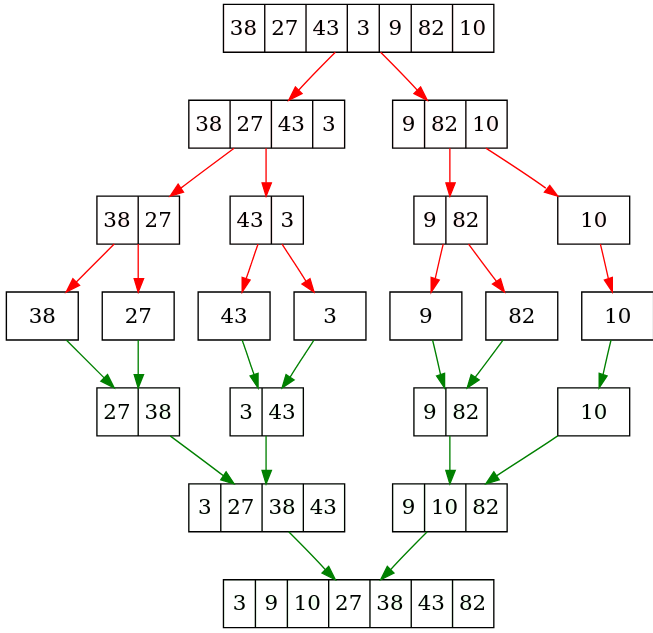
\includegraphics[width=200pt,height=150pt]{slike/mege.png} %merge-sort-example.png}
 	\label{fig:merge-sort}
 	\caption{Sortiranje niza spajanjem pomoću Podijeli-pa-zavladaj paradigme: korak po korak}
 \end{figure}


\begin{example}
	(\textbf{\textit{Množenje cijelih brojeva}}). Poznati algoritam za množenje dva $n$-cifrena broja, koji se uči u osnovnoj školi i zasniva se na množenju cifru po cifru, ima vremensku složenost $O(n^2)$. Konstruisati efikasniji algoritam zasnovan na paradigmi \emph{podijeli pa zavladaj} za problem množenja dva cijela broja.
\end{example}

\begin{solution}
	
	Radi jednostavnosti, bez smanjenja opštosti, pretpostavimo da su ulazni brojevi zapisani u binarnom obliku i da imaju isti broj cifara. Neka su dati brojevi $x$ i $y$, svaki dužine $n$ bitova. Podijelimo ih na lijevu i desnu polovinu: $
	x = x_1 2^{n/2} + x_2,
	\qquad
	y = y_1 2^{n/2} + y_2,
	$ gdje $x_1$, $x_2$, $y_1$ i $y_2$ sadrže $n/2 (\pm 1)$ bitova. 	Tada vrijedi
	
	$
	xy = (x_1 2^{n/2} + x_2)\cdot (y_1 2^{n/2} + y_2) =$ 
	$x_1y_1 2^n
	+
	(x_1y_2 + x_2y_1)2^{n/2}
	+
	x_2y_2.
	$
	
	Na osnovu ove formule potrebno je izračunati četiri proizvoda brojeva dužine $ \approx n/2$: $
	x_1y_1,\quad
	x_1y_2,\quad
	x_2y_1,\quad
	x_2y_2.
	$
	
	Rekurzija složenosti tada ima oblik $T(n)=4T(n/2)+O(n),$ pa prema Master teoremi dobijamo $T(n)=O(n^{\log_2 4})=O(n^2),$	što ne predstavlja poboljšanje u odnosu na klasični algoritam.
	
	Da bismo smanjili broj rekurzivnih množenja, koristimo sljedeću ideju:
	
	\begin{enumerate}
		\item Izračunamo $[
		z_1=x_1y_1]$.
		\item Izračunamo
		\[
		z_2=x_2y_2.
		\]
		\item Izračunamo $
		z_3=(x_1+x_2)(y_1+y_2).$
		
	\end{enumerate}
	
	Tada važi $z_3-z_1-z_2=
	x_1y_2+x_2y_1, $ 	pa se mješoviti član može dobiti bez dodatnih množenja. Prema tome, $xy=z_1 2^n	+	(z_3-z_1-z_2)2^{n/2} + z_2.$
	
	Na ovaj način broj rekurzivnih množenja smanjuje se sa četiri na tri, pa rekurzija postaje $T(n)=3T(n/2)+O(n).$ Primjenom Master teoreme dobijamo $T(n)=O(n^{\log_2 3})
	\approx O(n^{1.585}),$ što je asimptotski brže od klasičnog algoritma množenja (Pogledati Primjer 1.13). Ovaj pristup poznat je kao \textit{Karacubinov algoritam} (eng. {Karatsuba multiplication algorithm}).
\end{solution}

\section{Algoritamska paradigma vraćanja unazad}

{Vraćanje unazad} predstavlja algoritamsku paradigmu zasnovanu na rekurzivnoj izgradnji rješenja korak po korak. Tokom konstrukcije rješenja algoritam u svakom koraku provjerava da li trenutno parcijalno rješenje može biti prošireno u validno konačno rješenje. Ukoliko se utvrdi da neki izbor narušava ograničenja problema ili ne može dovesti do dopustivog rješenja, algoritam odustaje od tog pravca pretrage i vraća se na prethodnu odluku kako bi ispitao druge mogućnosti.

Ova paradigma može se posmatrati kao unaprijeđena verzija pristupa grube sile. Dok algoritmi grube sile ispituju sva moguća rješenja, algoritmi vraćanja unazad nastoje što ranije eliminisati dijelove prostora pretrage za koje se može zaključiti da ne sadrže validno rješenje. Na taj način često se postižu značajne uštede u vremenu izvršavanja.

Osnovna ideja paradigme sastoji se u tome da se rješenje gradi inkrementalno, dodavanjem jedne komponente u svakom koraku. Nakon svakog proširenja parcijalnog rješenja provjerava se da li ono i dalje zadovoljava uslove problema. Ako je odgovor negativan, pretraga se vraća na prethodni korak i pokušava drugačiji izbor.

Paradigma vraćanja unazad posebno je pogodna za probleme kod kojih:

\begin{itemize}
	\item rješenje možemo graditi postepeno;
	\item nakon svakog koraka možemo provjeriti da li je parcijalno rješenje dopustivo;
	\item postoji veliki broj mogućih kombinacija koje treba sistematski istražiti.
\end{itemize}

Tipični primjeri primjene ove paradigme uključuju Problem osam dama, bojenje grafa, sudoku, problem ruksaka, generisanje permutacija i kombinacija sa određenim ograničenjima, te mnoge druge kombinatorne optimizacione probleme. Opšti pseudokod paradigme vraćanja unazad dat je Algoritmom~\ref{alg:backtrack}.

\begin{algorithm}
	\begin{algorithmic}[1]
		\Procedure{Backtrack}{$x$}
		
		\If{$x$ nije dopustivo parcijalno rješenje}
		\State \Return
		\EndIf
		
		\If{$x$ predstavlja potpuno rješenje}
		\State Sačuvaj ili obradi rješenje $x$
		\State \Return
		\EndIf
		
		\For{svaku moguću odluku $e$}
		\State \textsc{Backtrack}(proširi $x$ sa $e$)
		\EndFor
		
		\EndProcedure
	\end{algorithmic}
	\caption{Opšti obrazac paradigme vraćanja unazad.}
	\label{alg:backtrack}
\end{algorithm}

Implementacija ove paradigme prirodno vodi ka konstrukciji \textit{stabla stanja} (eng. \emph{state-space tree}). Svaki čvor stabla predstavlja jedno parcijalno rješenje, dok grane odgovaraju mogućim proširenjima tog rješenja. Rekurzivni pozivi algoritma odgovaraju obilasku ovog stabla. Kada se utvrdi da određena grana ne dovodi do validnog rješenja, dalji obilazak te grane se prekida, čime se izbjegava nepotrebno pretraživanje.

U najgorem slučaju algoritmi vraćanja unazad i dalje mogu imati eksponencijalnu vremensku složenost, jer je ponekad potrebno istražiti veoma veliki broj mogućih kombinacija. Ipak, zahvaljujući ranom odbacivanju nedopustivih parcijalnih rješenja, oni su u praksi često znatno efikasniji od pristupa grube sile.

    %https://www.programiz.com/dsa/backtracking-algorithm ==> primjer 1...
    
 \begin{example}
 	(\textbf{\emph{Problem $N$ kraljica}}). Neka je data šahovska ploča dimenzija $N \times N$. Postaviti $N$ kraljica na ploču tako da se nikoje dvije kraljice međusobno ne napadaju. Riješiti problem primjenom paradigme vraćanja unazad.
 \end{example}
 
 \begin{solution}
 	
 	Posmatrajmo najpoznatiju varijantu ovog problema, problem osam kraljica ($N=8$). Jedno dopustivo rješenje prikazano je na Slici~\ref{fig:8-queen-sol-example}.
 	
 	\begin{figure}[H]
 		\centering
 		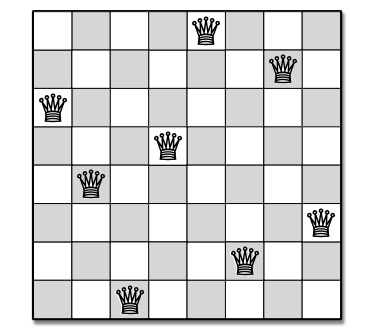
\includegraphics[width=200pt,height=180pt]{slike/n-queen-problem.png}
 		\caption{Primjer jednog rješenja problema osam kraljica.}
 		\label{fig:8-queen-sol-example}
 	\end{figure}
 	
 	Pošto se dvije kraljice ne smiju nalaziti u istom redu, svako rješenje možemo predstaviti nizom dužine $N$. Element na poziciji $i$ označava kolonu u kojoj je postavljena kraljica u $i$-tom redu šahovske ploče. Na primjer, raspored kraljica prikazan na Slici~\ref{fig:8-queen-sol-example} može se predstaviti nizom $
 	[5, 7, 1, 4, 2, 8, 6, 3]. $	Vrijednost na svakoj poziciji određuje kolonu u kojoj se smiješta kraljica u odgovarajući red.
 	
 	Algoritam vraćanja unazad započinje od praznog rješenja. U svakom koraku pokušava se postaviti nova kraljica u naredni red šahovske ploče. Drugim riječima, parcijalno rješenje se proširuje dodavanjem jedne nove komponente, odnosno izborom kolone u kojoj će se nalaziti kraljica u trenutno obrađivanom redu. Nakon svakog dodavanja provjerava se da li novopostavljena kraljica napada neku od prethodno postavljenih kraljica. Konflikt postoji ukoliko se dvije kraljice nalaze:
 	
 	\begin{itemize}
 		\item u istoj koloni;
 		\item na istoj glavnoj dijagonali;
 		\item na istoj sporednoj dijagonali.
 	\end{itemize}
 	
 	Ako se utvrdi postojanje konflikta, trenutno parcijalno rješenje ne može biti dio nijednog dopustivog konačnog rješenja. U tom slučaju algoritam odbacuje posljednji izbor, vraća se na prethodni nivo pretrage i pokušava postaviti kraljicu u neku drugu kolonu istog reda.
 	
 	Proces se nastavlja sve dok:
 	
 	\begin{itemize}
 		\item ne bude konstruisano dopustivo rješenje dužine $N$, čime su kraljice uspješno postavljene u sve redove šahovske ploče; ili
 		\item ne budu iscrpljene sve mogućnosti pretrage, kada zaključujemo da rješenje ne postoji.
 	\end{itemize}
 	
 	Problem $N$ kraljica predstavlja jedan od najpoznatijih primjera primjene paradigme vraćanja unazad, jer omogućava veoma efikasno odbacivanje velikog broja parcijalnih rješenja koja ne mogu dovesti do validnog rasporeda kraljica.
 \end{solution}
 
   
Implementacija problema je data narednim k\^odom. 

\begin{minted}[fontsize=\footnotesize,scale=0.8]{python}
	
   def NQueens(niz, N):
       if len(niz) == N: # kompletno rješenje
               return niz
       else:
              for col in range(N):
                  kandidat = niz + [col]
                  if valid(kandidat):
                      rezultat = NQueens(kandidat, N)
                      if rezultat is not None:
                          return rezultat
              return None

#main
N = 8
sol = NQueens([], N)       
if sol != None:
   print("Rješenje je: ", sol)
else:
   print("Nema rješenja") #npr. za N=3
   
\end{minted}
%%https://codeahoy.com/learn/recursion/ch10/
\begin{figure}
	\centering
	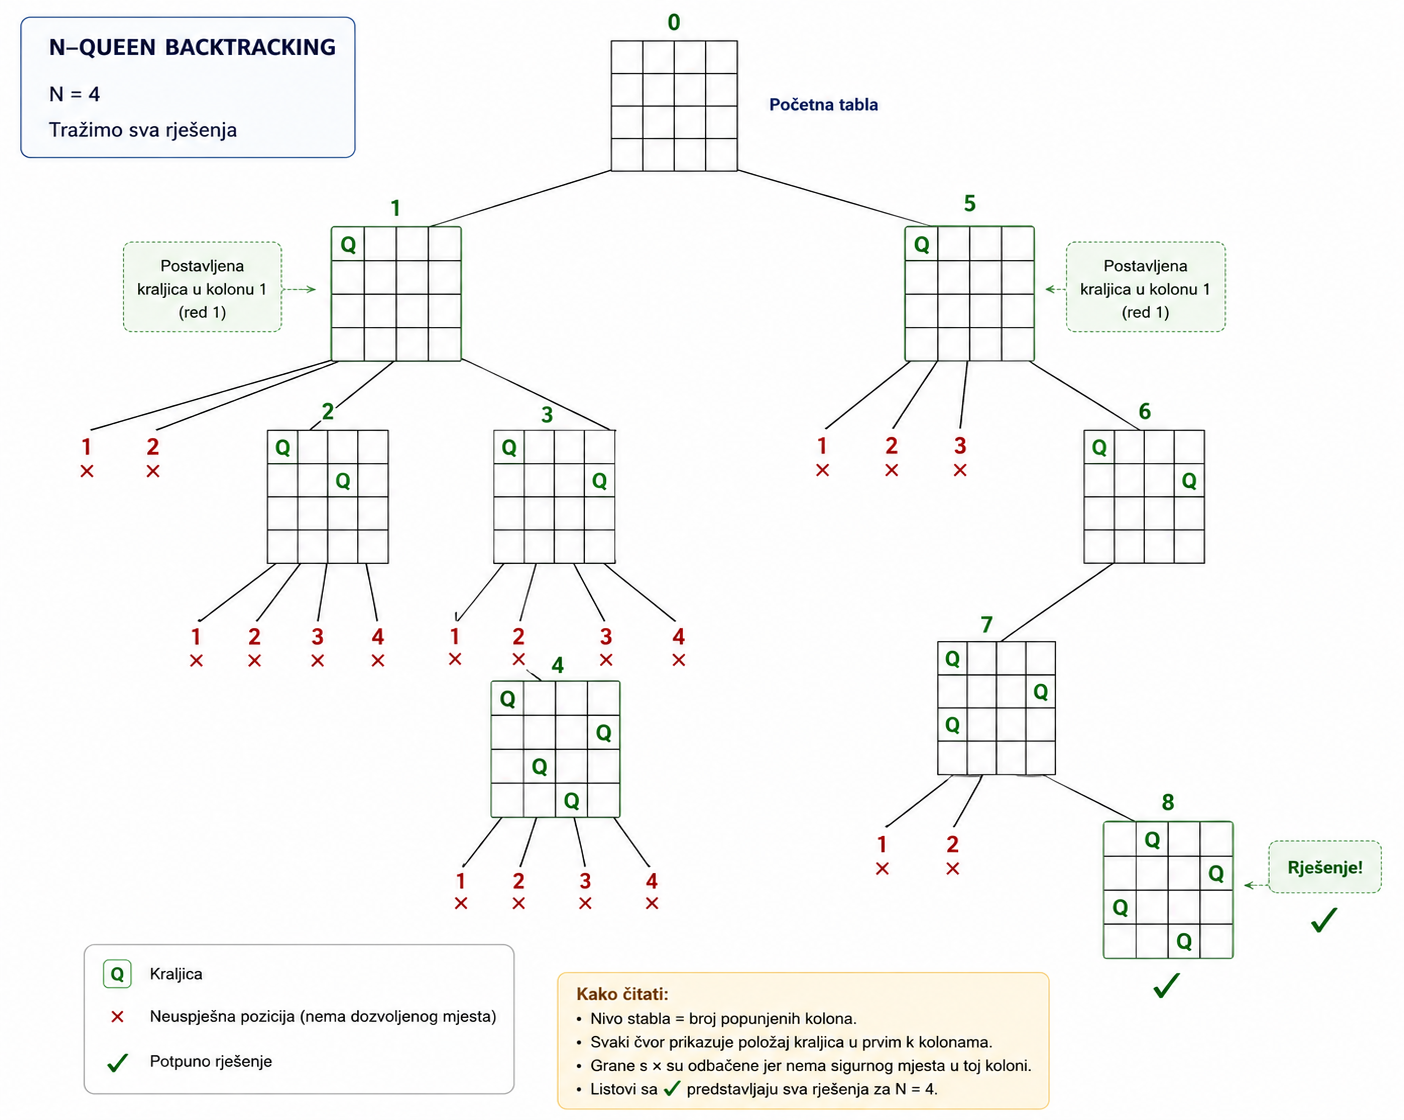
\includegraphics[width=350pt, height=280pt]{slike/n-queen-backtracking.png} %recursion-tree-backtracking-n-queens-1.png}
	\caption{Primjer stabla stanja formiranog algoritmom vraćanja unazad za problem 4 kraljice.}
\end{figure}
%\protect\footnotemark\footnotetext{Slika sa linka \url{https://towardsdatascience.com/genetic-algorithm-vs-backtracking-n-queen-problem-cdf38e15d73f}}

Napomenimo da ovdje nismo prikazali implementaciju funkcije \texttt{valid}(), koja vraća \textit{True} ako su pozicije kraljica  validne, u protivnom vraća \textit{False}. Ovo ostavljamo čitaocu kao zadatak za vježbanje. 


\end{solution}


    
 % Što se tiče problema koje ova paradigma rješava, dijelimo ih na tri tipa:
  %\begin{itemize}
  %	\item   \textit{Problem odlučivanja} -- U ovom slučaju tražimo izvodljivo rješenje.
  %	\item   \textit{Problem optimizacije} – U ovome tražimo najbolje rješenje.
  %	\item   \textit{Problem enumeracije} – U ovome nalazimo sva izvodljiva rješenja.
  %\end{itemize}


%https://codeahoy.com/learn/recursion/ch11/: THE SUM OF 4 SQUARES:

\begin{example}
	(\textbf{Problem sume 4 kvadrata}). Lagranžova teorema o 4 kvadrata kaže da se svaki prirodni broj može napisati kao zbir četiri broja koji su kvadrati nekih brojeva. Neka je dat broj $n$. Naći četiri kvadratna broja koji u zbiru daju broj $n$ pomoću algoritma vraćanja unazad.	Npr. za $n=2000$, vrijedi $1764 + 196 + 36 + 4 = 2000. $
\end{example}

\begin{solution}
	Rješenje problema predstavlja četvorka $sol = (a, b, c, d)$ prirodnih brojeva, tako da vrijedi $a^2 + b^2 + c^2 + d^2 = n$. Ideja rekurzije je odabrati svaki  od brojeva jedan po jedan, dok ne nađemo četvorku koja odgovara uslovima zadatka. Svaki put kada dodamo novi broj $x$ u rješenje \emph{sol}, naredni rekurzivni poziv ispituje trenutno zbir kvadrata brojeva u proširenom rješenju \emph{sol}. Ako vrijednost prelazi $n$, algoritam vrši vraćanje unazad i bira novog kandidata za proširivanje rješenja. 
	
 Implementacija algoritma vraćanja unazad za ovaj problem je dat narednim k\^odom.
 
 \begin{minted}[fontsize=\footnotesize,scale=0.8]{python}
from math import sqrt, pow

def FourSquareSum(sol):
	sum = 0
	for s in sol:
		sum += pow(s, 2)
	return sum

  def FourSumSquares(sol, n):
	if len(sol) == 4:
		if FourSquareSum(sol) == n:
			print(sol)
			return 
	else:
		for i in range(1, int(sqrt(n))+2):
			solI = sol + [i]
			sum_sol_i = FourSquareSum(solI)
			if sum_sol_i <= n-(4-len(solI)): # else backtrack  
				FourSumSquares(solI, n) 
  # poziv metode
  FourSumSquares([], 20)
 \end{minted}
	
	Kao što primijećujemo u prethodnom kodu, ako je \emph{sol} kardinalnosti 4, i ako je zbir kvadrata njegovih elemenata jednak $n$, ispisujemo \emph{sol} kao rješenje. U protivnom, ako je $|sol|<4$, (parcijalno) rješenje \emph{sol} proširujemo ubacujući naredni broj (varijabla $i\in \{1, \ldots, \lfloor\sqrt{n} \rfloor + 1 \}$), dobijajući niz \emph{solI}.  Ako je zbir kvadrata elemenata iz \emph{sol} veći od $n-(4 - |solI|)$, ovakva ekstenzija nikada neće voditi ka rješenju koje zadovoljava uslove zadatka, pa pretraga ide unazad, rekurzivno,  ispitujući druge kandidate za proširenje trenutnog rješenja \emph{sol}. Inicijalno, rješenje \emph{sol} je predstavljeno praznim nizom.
	 
\end{solution}
 
 
\section{Pohlepni algoritmi}

\textit{Pohlepni algoritmi}  predstavljaju algoritamsku paradigmu u kojoj se u svakom koraku donosi lokalno najbolja odluka o proširenju parcijalnog rješenja prema unaprijed definisanom kriterijumu. Osnovna ideja je da se problem rješava nizom lokalno optimalnih izbora, uz pretpostavku da će takvi izbori dovesti do kvalitetnog, a ponekad i optimalnog globalnog rješenja.

Za razliku od algoritama vraćanja unazad ili dinamičkog programiranja, pohlepni algoritmi ne preispituju ranije donesene odluke. Jednom kada se neka komponenta uključi u rješenje, ona se više ne uklanja niti mijenja. Zbog toga su pohlepni algoritmi obično veoma efikasni, ali ne garantuju uvijek pronalazak optimalnog rješenja.

Drugim riječima, algoritam u svakom koraku bira opciju koja je trenutno najpovoljnija, bez razmatranja mogućih posljedica tog izbora na buduće korake. Zbog toga, uspješnost ovog pristupa zavisi od strukture problema. Za određene klase problema može se dokazati da lokalno optimalni izbori vode ka globalno optimalnom rješenju, dok kod drugih problema pohlepni pristup daje samo aproksimativna/heuristička rješenja. 

U neformalnom smislu, pohlepni algoritam započinje od praznog ili djelimično izgrađenog rješenja i zatim ga iterativno proširuje komponentama koje imaju najveću trenutnu korist. Proces se nastavlja sve dok se ne dobije potpuno rješenje ili dok se ne iscrpe sve mogućnosti za dopustivo proširenje.

Opšta shema pohlepnog pristupa prikazana je Algoritmom~\ref{alg:greedy-algorithm}. Ulaz u algoritam čine instanca problema $\mathcal{P}$ i pohlepna funkcija $g$, koja procjenjuje kvalitet mogućih proširenja trenutnog rješenja.

U svakoj iteraciji izvršavaju se sljedeći koraci:

\begin{itemize}
	\item određuje se skup svih komponenti koje na dopustiv način mogu proširiti trenutno parcijalno rješenje;
	\item među njima se bira komponenta sa najboljom vrijednošću pohlepne funkcije;
	\item izabrana komponenta se dodaje trenutnom rješenju.
\end{itemize}

Proces se ponavlja sve dok postoji barem jedna komponenta koja može dopustivo proširiti trenutno rješenje. Nakon toga algoritam vraća konstruisano rješenje.

\begin{algorithm}
	\begin{algorithmic}[1]
		\State \textbf{Ulaz:} instanca problema, pohlepna funkcija $g$
		\State \textbf{Izlaz:} (aproksimativno) rješenje problema
		\State $x \gets$ inicijalno parcijalno rješenje
		\State $\mathcal{C} \gets$ skup dopustivih proširenja rješenja $x$
		
		\While{$\mathcal{C} \neq \emptyset$}
		\State $e \gets$ lokalno najbolja komponenta iz $\mathcal{C}$ shodno vrijednosti funkc. $g$
		\State $x \gets$ proširi rješenje $x$ komponentom $e$
		\State $\mathcal{C} \gets$ odredi nova dopustiva proširenja rješenja $x$
		\EndWhile
		
		\State \Return $x$
	\end{algorithmic}
	\caption{Opšta shema pohlepnog algoritma.}
	\label{alg:greedy-algorithm}
\end{algorithm}

Da bi se neki problem mogao rješavati pohlepnim pristupom, potrebno je definisati:

\begin{enumerate}
	\item skup komponenti od kojih se gradi rješenje;
	\item reprezentaciju parcijalnog rješenja;
	\item kriterijum za izbor sljedeće komponente, odnosno pohlepnu funkciju;
	\item uslove dopustivosti proširenja parcijalnog rješenja.
\end{enumerate}

Najpoznatiji primjeri primjene pohlepnih algoritama uključuju problem izbora aktivnosti, konstrukciju Hafmanovog stabla, algoritme za pronalaženje minimalnog razapinjućeg stabla (Kruskalov i Primov algoritam), te određene varijante problema najkraćih puteva, kao što je Dijkstrin algoritam za grafove sa nenegativnim težinama grana.

Glavna prednost pohlepnih algoritama jeste njihova jednostavnost implementacije i mala vremenska složenost. Međutim, njihov osnovni nedostatak je što lokalno najbolji izbor ne mora uvijek voditi globalno optimalnom rješenju. Zbog toga je prije primjene ove paradigme potrebno dokazati da problem posjeduje tzv. \emph{pohlepno svojstvo} (eng. \emph{greedy-choice property}), odnosno da optimalno rješenje može biti izgrađeno nizom lokalno optimalnih odluka.


Ovu paradigmu koristimo kada je potrebno pronaći rješenje zadovoljavajućeg kvaliteta u relativno kratkom vremenu, uz jednostavnu implementaciju algoritma. Zbog svoje efikasnosti i konceptualne jednostavnosti, pohlepni pristup često predstavlja prvi korak u rješavanju složenih kombinatornih i optimizacionih problema.

Pohlepni algoritmi se takođe često koriste za generisanje početnih rješenja koja se kasnije dodatno poboljšavaju naprednijim metodama, kao što su lokalna pretraga, metaheuristike ili egzaktni algoritmi. U tom smislu, oni pružaju korisnu polaznu osnovu za razumijevanje strukture problema i procjenu kvaliteta rješenja koja se mogu dobiti korištenjem jednostavnih konstruktivnih heuristika.

U nastavku prikazujemo nekoliko primjera primjene pohlepnih algoritama na različite kombinatorne probleme.

\begin{example}
	(\textbf{\emph{Problem razmjenjivanja novca}}).
	
	Neka je dato $X$ KM i skup apoena $x_1, x_2, \ldots, x_k$, pri čemu je svaki apoen dostupan u neograničenoj količini. Pretpostavimo da su $X$ i svi apoeni prirodni brojevi. \\
	
	
	Na koji način razmijeniti iznos $X$ tako da ukupan broj novčanica i kovanica bude minimalan? Problem riješiti primjenom pohlepnog pristupa.
\end{example}

\begin{solution}
	
	Definišimo najprije strukturu rješenja. Svako rješenje može se predstaviti $k$-torkom $(p_1,p_2,\ldots,p_k),$ gdje $p_i$ označava broj iskorištenih apoena vrijednosti $x_i$. Rješenje je dopustivo ukoliko vrijedi $\sum_{i=1}^{k} p_i x_i = X.$
	
	Parcijalno rješenje predstavlja djelimično formiranu kombinaciju apoena $(p_1,p_2,\ldots,p_s), s \leq k,$ za koju vrijedi $\sum_{i=1}^{s} p_i x_i \leq X.$ 	Takvo rješenje se može dalje proširivati dodavanjem novih apoena.
	
	Osnovna ideja pohlepnog algoritma jeste da se u svakom koraku bira najveći apoen koji ne premašuje preostali iznos koji treba razmijeniti. Nakon izbora apoena uzima se maksimalan mogući broj novčanica ili kovanica tog apoena, a zatim se isti postupak ponavlja za preostali iznos.\\ 
	
	Pretpostavimo da su apoeni sortirani opadajuće: $ x_1 > x_2 > \cdots > x_k.$
	
	Neka je $X' = X - \sum_{j=1}^{s} p_j x_j$ preostali iznos koji još treba razmijeniti. Tada se bira najveći apoen $x_i$ za koji važi $x_i \leq X',$ a broj njegovih pojavljivanja određuje se kao $p_i=\left\lfloor \frac{X'}{x_i}\right\rfloor.$  	Na taj način parcijalno rješenje se proširuje novom komponentom, nakon čega se ažurira vrijednost preostalog iznosa. Postupak se ponavlja sve dok preostali iznos ne postane nula.
	
	%Za standardne novčane sisteme (npr. konvertibilna marka, euro ili američki dolar) ovakav pohlepni postupak daje optimalno rješenje, odnosno minimalan broj novčanica i kovanica. Međutim, za proizvoljno definisane skupove apoena to ne mora uvijek biti slučaj, pa je u takvim situacijama potrebno koristiti naprednije algoritamske tehnike.
\end{solution}

Implementacija algoritma ovog problema  je data u nastavku.
	 \begin{minted}[fontsize=\footnotesize,scale=0.75]{python}
	 def razmijeni(P, X):
	 	rjesenje = []
	 	i = 0
	 	usitnjeno, brojNovcanica = 0, 0
	 	sortApoeni = sorted(P) # sort apoene opadajuće
	 	while i <  n and usitnjeno < X :
	 		pi = (X - usitnjeno) // P[i]  #br. novcanica sortApoeni[i]
	 		if pi > 0:
	 			usitnjeno = usitnjeno + pi * sortApoeni[i]
	 			brojNovcanica = brojNovcanica + pi
	 		i = i + 1
	 	if usitnjeno == X:
	 		return brojNovcanica
	 	else:
	 		return -1 # ne može se usitniti
	 \end{minted} 
\end{solution}

\textbf{Vremenska složenost}. Sortiranje algoritma zahtijeva $O(n \log n)$ vreme\-na. Dalje, glavna petlja se izvršava u $O(n)$ vremenu, odakle slijedi da je ukupno vrijeme izvršavanja algoritma jednako $O(n \log n)$, što je, svakako, polinomi\-jalno. Za kanonske sisteme apoena, kakvi se koriste u većini standardnih valuta, pohlepni algoritam daje optimalno rješenje.   %Napomenimo da ovakvom strategijom garantujemo nalazak optimalnog rje\-šenja problema, (ili utvrđujemo da rješenje ne postoji) što se formalno može i pokazati. 


\begin{example}
	(\textbf{\emph{Razlomljeni problem ruksaka}}). Ovaj problem predstavlja relaksiranu verziju klasičnog problema ruksaka. Za razliku od standardne varijante, gdje se svaki proizvod mora uzeti u cijelosti ili se uopšte ne uzima, ovdje je dozvoljeno uzeti proizvoljan dio proizvoda. Takva pretpostavka ima smisla za proizvode koji se mogu dijeliti, kao što su šećer, brašno, ulje ili gorivo. \\
	
	Dat je skup proizvoda, pri čemu svaki proizvod $i$ ima težinu $w_i$ i vrijednost $p_i$, kao i ruksak kapaciteta $C$. Potrebno je odrediti koje proizvode, odnosno koje njihove dijelove, treba smjestiti u ruksak tako da ukupna vrijednost bude maksimalna, uz poštovanje ograničenja kapaciteta.
	
	Problem riješiti primjenom pohlepnog pristupa.
\end{example}

\begin{solution}
	
	Posmatrajmo instancu problema $n=3,
	w=[10,20,30],
	p=[60,100,120],$ 	pri čemu je kapacitet ruksaka jednak $C=50$.
	
	Optimalno rješenje dobija se tako što se prvi i drugi proizvod uzimaju u potpunosti, dok se od trećeg proizvoda uzima samo dio. Ukupna težina prva dva proizvoda iznosi $10+20=30$, pa u ruksaku ostaje još $20$ jedinica slobodnog prostora. Kako treći proizvod ima težinu $30$, moguće je uzeti samo njegov dio $\frac{20}{30}=\frac{2}{3}.$  Ukupna vrijednost ruksaka tada iznosi 	$60 + 100 + \frac{2}{3}\cdot 120 = 240.$ \\
	\medskip
	\textit{Struktura rješenja.}	Rješenje predstavljamo vektorom $c=(c_1,c_2,\ldots,c_n),$ gdje je $0\leq c_i\leq 1$ udio proizvoda $i$ koji se nalazi u ruksaku. Pri tome mora važiti ograničenje kapaciteta $	\sum_{i=1}^{n} c_i w_i \leq C.$
	
	\medskip
	
	\textit{Parcijalna rješenja i komponente rješenja.}
	Parcijalno rješenje čini bilo koji skup već odabranih proizvoda i njihovih udjela koji ne narušavaju kapacitet ruksaka. Komponente rješenja predstavljaju proizvodi koji još nisu razmatrani i koji mogu dopustivo proširiti trenutno rješenje.
	
	\medskip
	
	\textit{Pohlepna funkcija.}
	Ključna ideja je da prednost dajemo proizvodima koji ostvaruju najveću vrijednost po jedinici težine. Za svaki proizvod računamo omjer $
	\rho_i=\frac{p_i}{w_i}.$  Vrijednost $\rho_i$ predstavlja profit ostvaren po jedinici zauzetog kapaciteta i prirodno određuje prioritet proizvoda. Najprije se sortiraju proizvode opadajuće prema vrijednosti $\rho_i$. Neka je nakon sortiranja redoslijed proizvoda označen indeksima $1,2,\ldots,n.$
	
	Algoritam zatim prolazi kroz proizvode tim redoslijedom. Za svaki proizvod uzima se najveći mogući dio koji još može stati u preostali kapacitet ruksaka. Ako proizvod može stati u cijelosti, postavlja se $c_i=1$. U suprotnom, uzima se upravo onaj dio koji popunjava preostali kapacitet: $c_i=  \frac{\text{preostali\_kapacitet}}{w_i}.$  Nakon toga je ruksak popunjen i algoritam se završava.
	
	\medskip
	
	Pohlepni algoritam za razlomljeni problem ruksaka ima vremensku složenost $O(n\log n)$, koja potiče od sortiranja proizvoda (prema omjeru $\frac{p_i}{w_i}$). Za razliku od klasičnog problema ruksaka, kod ove relaksirane varijante može se dokazati da opisani pohlepni pristup uvijek daje optimalno rješenje.
\end{solution}


  Implementacija algoritma je data naredim k\^odom. 
   
   \begin{minted}[fontsize=\footnotesize,scale=0.8]{python}
  def fraction(i):
  	return P[i]/ W[i]
  
  def fraction_knapsack():
  
  	products = [i for i in range(len(W))] #lsit of prods
  	products.sort(key = fraction, reverse=True)
  	#print(products)
  	current_C = C
  	sol, parts = [], []

  	for i in products:
  
  		part = min(current_C / W[i], 1)
  		if part > 0:
  			sol.append(i)
  			parts.append(part)
  			current_C -= part * W[i]
  
  		else: # knapsack filled
  			return sol, parts
          return sol, parts
    #instanca: 
    W = [10, 20, 30]
    P = [60, 100, 120]
    C = 50
    sol, parts = fraction_knapsack()
    print(sol, " parts: ", parts)
  
   \end{minted}

\textit{Kompleksnost algoritma}.  Najviše vremena je utrošeno na sortiranje proi\-zvoda, što iznosi $O(n \log n)$ vremena. Dalje, u glavnoj petlji, koja se vrti najviše $n$ puta,  svaka iteracija se izvršava u konstantnom vremenu. Dakle, vrijeme izvršavanja petlje je $O(n)$. Prema tome, algoritam se izvršava u $O(n \log n)$ vremenu. %Napomenimo da ovaj algoritam takođe garantuje nalazak optimalnog rješenja, što se formalno može i pokazati. 
\end{solution}


\begin{example}
	(\textbf{\emph{Problem pokrivanja skupa}}). 	Neka je dat konačan skup $X$ i familija njegovih podskupova
	$\mathcal{F}\subseteq P(X)$, pri čemu važi 	$\bigcup_{F\in \mathcal{F}} F = X.$ Potrebno je pronaći podfamiliju $S\subseteq \mathcal{F}$ minimalne kardinalnosti takvu da vrijedi $\bigcup_{A\in S} A = X.$ \\
	
	Drugim riječima, cilj je odabrati što manji broj skupova iz familije $\mathcal{F}$ tako da njihova unija pokrije sve elemente skupa $X$. Problem riješiti primjenom pohlepnog pristupa.
\end{example}

\begin{solution}
	
	Posmatrajmo instancu $
	X=\{1,2,3,4,5\},$ i familiju skupova  $
	\mathcal{F}=
	\big\{
		\{1,2,3\},
		\{1,4\},
		\{2,4,5\},
		\{2,3\},
		\{4,5\},
		\{1,5\}
		\big\}.$
	
	Jedno optimalno rješenje je $S= \big\{
		\{1,2,3\},
		\{2,4,5\}
		\big\},$	jer unija skupova u rješenju pokriva čitav skup $X$, a pri tome je $|S|=2.$
	
	Problem pokrivanja skupa ima brojne praktične primjene. Na primjer, može predstavljati zadatak izbora minimalnog broja stručnjaka u komisiji tako da svaka potrebna oblast bude zastupljena barem jednim članom komisije. Slične primjene javljaju se u planiranju mreža senzora, raspoređivanju resursa i izboru lokacija za pružanje usluga.
	
	\medskip
	
	\textit{Struktura rješenja.}	Rješenje problema je predstavljeno podfamilijom skupova $S\subseteq \mathcal{F}$	takva da njihova unija pokriva sve elemente skupa $X$.
	
	\medskip
	
	\textit{Parcijalna rješenja i komponente rješenja.}
	Parcijalno rješenje predstavlja proizvoljna podfamilija
    $S\subseteq \mathcal{F},$  	koja ne mora nužno pokrivati čitav skup $X$.  Komponente koje mogu proširiti trenutno rješenje jesu svi skupovi iz familije $\mathcal{F}\setminus S.$ Proširenje parcijalnog rješenja vrši se dodavanjem novog skupa: $
	  S' = S \cup {C}, C\in \mathcal{F}\setminus S.$
	
	\medskip
	
	\textit{Pohlepna funkcija.}	Neka trenutno parcijalno rješenje $S$ pokriva skup elemenata $ X_S= \bigcup_{A\in S} A.$	Preostali nepokriveni elementi dati su skupom $
	X\setminus X_S.
	$   Intuitivno, najbolji izbor u datom koraku jeste skup koji pokriva najveći broj trenutno nepokrivenih elemenata. Zbog toga definišemo pohlepnu funkciju 	$$ g(S,C)= \left| C\cap (X\setminus X_S) \right|,$$
 koja mjeri broj novih elemenata koje skup $C$ doprinosi trenutnom rješenju.	U svakoj iteraciji bira se skup $ C^* = \arg\max_{C\in \mathcal{F}\setminus S}
	g(S,C),
	$ odnosno skup koji pokriva najveći broj još nepokrivenih elemenata.
	
	\medskip
	
	Pohlepni algoritam započinje praznim rješenjem $S=\emptyset$. U svakoj iteraciji bira skup $C^*$ koji maksimizuje funkciju $g$, dodaje ga u rješenje i ažurira skup pokrivenih elemenata. Postupak se ponavlja sve dok svi elementi skupa $X$ ne budu pokriveni ili ne postoji više skupova koji se mogu dodati u rješenje.  Važno je naglasiti da opisani pohlepni algoritam ne garantuje uvijek optimalno rješenje. Ipak, zbog svoje jednostavnosti i efikasnosti veoma je često korišten u praksi i predstavlja jednu od najpoznatijih aproksimativnih metoda za problem pokrivanja skupa.
	
	Radi efikasnije implementacije, umjesto samih skupova u rješenju se čuvaju odgovarajući indeksi unutar familije $\mathcal{F}$.
\end{solution}

Implementacija algoritma  je data u nastavku sljedećim k\^odom.

\begin{minted}[fontsize=\footnotesize,scale=0.8]{python}
	def g(X_S, C):
		return len((X.difference(X_S)).intersection(C))
	
	def cover_X():
		X_S = set(())
		S = [] # solution
	
		while(X_S != X):
			C_star = istar = None
			g_best = 0
	
			for i in range(len(F)):# iteration best-next
				if i  not  in S: 
					g_i = g(X_S, F[i])
					if g_best < g_i:
						g_best = g_i
						i_star = i
			X_S = X_S.union(F[i_star]) #update cover
			S.append(i_star)
		return  S            
	
	#instanca: 
	X = {1, 2, 3, 4, 5}
	F = [{1, 2, 3}, {1, 4}, {2, 4, 5}, {2, 3}, {4, 5}, {1, 5}]
	sol = []
	C = 50
	sol = cover_X()
	print(sol)
	
\end{minted}

\textit{Vremenska složenost}. Glavna \texttt{while}-petlja izvršava najviše $n$ iteracija. U unutrašnjoj \texttt{for}-petlji, koja se izvršava  $ |\mathcal{F}|$ puta, najskuplja operacija je poziv pohlepne funkcije \textit{g}, koja se izvršava u linearnom vremenu, tj. u $O(n)$. Dakle, kompleksnost čitave \texttt{for} petlje je $O(n \cdot  |\mathcal{F} |)$. Zajedno, kompleksnost algoritma je $O(n^2 \cdot  |\mathcal{F} |)$. Na osnovu dobijenog, zaključujemo da efikasnost algoritma najviše zavisi od veličine skupa $\mathcal{F}$. 

Napomenimo da ovako dizajniran algoritam ne garantuje nalazak opti\-malnog rješenja  kao u prethodna dva problema. Uzmimo npr. instancu $X= \{1, 2, 3, 4, 5, 6\}$, te $$\mathcal{F}= \{\{1,2\}, \{3, 4\}, \{4, 5\}, \{3, 6\}, \{5\}, \{6\} \}.$$   
  Prva iteracija u algoritmu će odabrati, prvi skup $\{1, 2\}$ i dodati ga u parcijalno rješenje. Naredna iteracija odabire skup $\{3, 4\}$. Nakon toga, bira se $\{4, 5\}$, pa $\{6\}$. Dakle, dobijeno rješenje je kardinalnosti 4. Međutim, ono očigledno ne predstavlja optimalno rječenje. 
  
  Optimalno rješenje je veličine 3 i dato je sa $\{ \{1, 2\}, \{3, 6\}, \{4,5\}\}$.  
	 
\end{solution}

\begin{example}
	(\textbf{\emph{Problem sekvencijalnog raspoređivanja poslova}}).
	
	Dat je skup poslova, pri čemu je za svaki posao poznat krajnji rok izvršavanja (eng. \emph{deadline}) i profit koji se ostvaruje ukoliko posao bude završen najkasnije do tog roka. Pretpostavimo da je za izvršavanje svakog posla potrebno tačno jedna jedinica vremena, te da svi poslovi mogu započeti od trenutka $t=0$.\\ 

	
	Potrebno je odabrati podskup poslova i odrediti njihov raspored izvršavanja tako da ukupan ostvareni profit bude maksimalan. Pri tome vrijedi ograničenje da se u svakoj jedinici vremena može izvršavati najviše jedan posao.	Problem riješiti primjenom paradigme pohlepnih algoritama.
\end{example}

\begin{solution}
	
	Posmatrajmo sljedeću instancu problema.
	
	\begin{center}
		\begin{tabular}{ccc}
			\emph{Posao} & \emph{Krajnji rok} & \emph{Profit} \\ \hline \hline 
			1 & 4 & 20 \\
			2 & 1 & 10 \\
			3 & 1 & 40 \\
			4 & 1 & 30 \\ \hline
		\end{tabular}
	\end{center}
	
	Optimalno rješenje u ovom slučaju čine poslovi $\{3,1\}$, čiji je ukupan profit jednak $40 + 20 = 60.$
	
	Posmatrajmo sada drugu instancu problema.
	
	\begin{center}
		\begin{tabular}{ccc}
			\emph{Posao} & \emph{Krajnji rok} & \emph{Profit} \\  \hline \hline
			1 & 2 & 100 \\
			2 & 1 & 19 \\
			3 & 2 & 27 \\
			4 & 1 & 25 \\
			5 & 3 & 15 \\ \hline
		\end{tabular}
	\end{center}
	
	Jedno optimalno rješenje dobija se izvršavanjem poslova $\{3,1,5\}$. Poslovi se mogu rasporediti u vremenske intervale tako da poštuju zadate rokove, pri čemu je ukupan profit $27 + 100 + 15 = 142.$
	
	\medskip
	
	Prva ideja za rješavanje ovog problema bila bi potpuna enumeracija svih podskupova poslova. Za svaki generisani podskup provjerila bi se dopustivost rasporeda i izračunao ostvareni profit. Međutim, broj mogućih podskupova jednak je $2^n$, pa takav pristup postaje neupotrebljiv već za umjerene vrijednosti $n$.
	
	Zbog toga razmatramo pohlepni pristup.
	
	\medskip
	
	\textit{Struktura rješenja.} Rješenje problema predstavlja skup odabranih poslova zajedno sa njihovim rasporedom izvršavanja. Rješenje je dopustivo ako:
	
	\begin{itemize}
		\item svaki odabrani posao bude završen najkasnije do svog krajnjeg roka;
		\item u svakom vremenskom trenutku bude izvršavan najviše jedan posao.
	\end{itemize}
	
	\medskip
	
	\textit{Parcijalno rješenje i njegovo proširenje.}
	Parcijalno rješenje predstavlja bilo koji dopustiv raspored dijela poslova. Komponente koje mogu proširiti parcijalno rješenje jesu poslovi koji još nisu raspoređeni, a koji se mogu dodati bez narušavanja ograničenja problema. 	Proširenje parcijalnog rješenja podrazumijeva dodavanje novog posla u neki slobodan vremenski interval tako da njegov krajnji rok ostane zadovoljen. Recimo, slobodan vremenski interval bi mogao biti onaj koji je najkasniji mogući a ne narušava ni krajnji rok izvršavanja konkretnog posla, niti postoji konflikt između poslova koji bi se simultano izvršavali u istom vremenskom intervalu. 
	
	\medskip
	
	\textit{Pohlepna funkcija.}
	Intuitivno je razumno dati prednost poslovima koji donose veći profit. Zbog toga se poslovi najprije sortiraju po profitu u opadajućem poretku.\\
	
	Neka je trenutno parcijalno rješenje označeno sa $I_s$. U svakoj iteraciji bira se neraspoređeni posao sa najvećim profitom. Ukoliko je moguće pronaći  slobodan vremenski interval prije krajnjeg roka, posao se dodaje u raspored. U suprotnom, posao se odbacuje i razmatra se naredni posao iz sortirane liste.  Da bi se ostavilo što više prostora za buduće poslove, odabrani posao se smiješta u \textit{posljednji} (najkasniji) slobodan vremenski interval koji ne prelazi njegov krajnji rok.
	
	\medskip
	
	Algoritam se može opisati sljedećim koracima:
	
	\begin{enumerate}
		\item Sortirati poslove po profitu u opadajućem poretku.
		\item Poštujući redoslijed sortiranja, idući od posla do posla, pronaći  (najkasniji) slobodan vremenski interval prije krajnjeg roka.
		\item Ako takav interval postoji, posao rasporediti u njega.
		\item U suprotnom, posao odbaciti i preći na drugi.
		\item Nakon razmatranja svih poslova vratiti dobijeni raspored.
	\end{enumerate}
	
	Pohlepni algoritam za ovaj problem izvršava se znatno brže od potpune enumeracije, a pritom daje optimalno rješenje. Ključna ideja sastoji se u tome da se najprofitabilniji poslovi raspoređuju što je moguće kasnije, čime se ostavlja maksimalna fleksibilnost za raspoređivanje preostalih poslova.
\end{solution}


Implementacija algoritma je data sljedećim k\^odom. 
 
 \begin{minted}[fontsize=\footnotesize,scale=0.8]{python}
 
 def ProfitSort(i):
 	return Profit[i]
 
 # možemo li dodati i-ti proizvod ili ne (-1) u I_s
 def find_next_interval(I_s_covered, i):
 
 	for index, covered in enumerate(I_s_covered):
 	    rev_index = len(I_s_covered)-index
 		if rev_index > Deadline[i]:
 			return continue
 		if covered == False:
 			return rev_index
 	return -1       
 
 def sequnetial_scheduling():
 
 	I_s_covered = [False] *  max(Deadline) 
 	I_s = []
 	#sortiranje jobs u odnosu na Profit (preprocessing):
 	Jobs.sort(key=ProfitSort, reverse=True)

 	for i in Jobs:
 
 		interval = find_next_interval(I_s_covered, i)
 		if interval >= 0: #nadjena (dopustiv) interval:
 			I_s_covered[interval] = True #zauzet
 			I_s.append(i)
 
 	return I_s, sum([ Profit[I_s[i]]  for i in range(len(I_s)) ])
 
 #main:
 num_jobs = 5
 Jobs = [i for i in range(num_jobs)]
 Deadline = [2, 1, 2, 1, 3]
 Profit = [100, 19, 27, 25, 15]
 # izvrsavanje algoritma:
 I_s, profit = sequnetial_scheduling()
 print(I_s, " profit: ", profit)
 \end{minted}

\textit{Vremenska kompleksnost}. Sortiranje poslova se odvija u $O(n \log n)$. Dalje, glavna \texttt{while}-petlja se sastoji od $n$ iteracija. U svakoj iteraciji, najskuplja operacija je poziv funkcije \texttt{find\_next\_interval} koja se izvršava u vremenu $O(n)$. Prema tome,   glavna petlja se izvršava u $O(n^2)$. Zaključujemo da se implementacija algoritma izvršava u $O(n^2)$. 

Napomenimo da se može pokazati da ovaj pohlepni algoritam garantuje nalazak optimalnog rješenja.

\section{Dinamičko programiranje}

\textit{Dinamičko programiranje} predstavlja algoritamsku tehniku namijenjenu efikasnom rješavanju problema koji imaju dvije ključne karakteristike:

\begin{itemize}
	\item \textit{preklapajuće podprobleme} (eng. \emph{overlapping subproblems});
	\item \textit{optimalnu podstrukturu} (eng. \emph{optimal substructure}).
\end{itemize}

Pod \textit{preklapajućim podproblemima} podrazumijevamo situaciju u kojoj se isti podproblem javlja više puta tokom rješavanja većeg problema. Umjesto da se rješenje podproblema svaki put iznova računa, ono se  jednom izračuna i rezultat se čuva za kasniju upotrebu. Svojstvo \textit{optimalne podstrukture} znači da se optimalno rješenje početnog problema može konstruisati kombinovanjem optimalnih rješenja njegovih podproblema. Drugim riječima, rješavanje podproblema na optimalan način vodi ka optimalnom rješenju originalnog problema.

Osnovna ideja dinamičkog programiranja sastoji se u izbjegavanju više\-strukog rješavanja istih podproblema. Umjesto ponovnog računanja, rezultati se pohranjuju u memoriju i po potrebi ponovo koriste. Ovaj postupak naziva se \textit{memoizacija}.

Memoizacija značajno poboljšava efikasnost rekurzivnih algoritama, jer se svaki podproblem rješava najviše jednom. Naravno, cijena ovog ubrzanja jeste dodatni memorijski prostor potreban za pohranjivanje već izračunatih rezultata.

\medskip

Da bismo primijenili dinamičko programiranje na određeni problem, potrebno je:

\begin{itemize}
	\item formulisati problem u obliku rekurzivne relacije koja ga razlaže na manje podprobleme;
	\item identifikovati podprobleme čija se rješenja ponavljaju;
	\item sačuvati rješenja podproblema u odgovarajućoj memorijskoj strukturi radi njihove ponovne upotrebe.
\end{itemize}

\subsection{Memoizacija (pristup odozgo prema dolje)}

Memoizacija (eng. \emph{top-down approach}) predstavlja implementaciju dinamičkog programiranja zasnovanu na rekurziji. Algoritam se izvršava na isti način kao i obična rekurzija, ali se rezultati već riješenih podproblema pohranjuju u pomoćnu strukturu podataka (npr. rječnik ili tabelu).

Prilikom svakog novog poziva prvo se provjerava da li je odgovarajući podproblem već riješen. Ukoliko jeste, prethodno izračunato rješenje se odmah vraća bez dodatnog računanja.

\medskip

Prednosti memoizacije su:

\begin{itemize}
	\item jednostavna implementacija kada je rekurzivna formulacija problema prirodna;
	\item računanje samo onih podproblema koji su zaista potrebni.
\end{itemize}

Nedostatak je dodatni trošak rekurzivnih poziva i memorije steka.

\subsection*{Tabuliranje (pristup odozdo prema gore)}

Drugi način implementacije dinamičkog programiranja naziva se \textit{tabuliranje} (eng. \emph{tabulation}) ili pristup \textit{odozdo prema gore} (eng. \emph{bottom-up approach}).

Kod ovog pristupa problem se ne rješava rekurzivno. Umjesto toga, prvo se izračunavaju rješenja najmanjih podproblema, a zatim se ona sistematski koriste za konstruisanje rješenja većih podproblema, sve do konačnog rješenja.  Rezultati se pohranjuju u tabelu (najčešće niz ili matricu), po čemu je ovaj pristup i dobio naziv.  Prednosti tabuliranja su:

\begin{itemize}
	\item nema troška rekurzivnih poziva;
	\item nema opasnosti od prekoračenja steka;
	\item često postiže bolje praktične performanse od memoizacije.
\end{itemize}

Sa druge strane, tabuliranje ponekad zahtijeva računanje i onih podproblema koji možda nisu neophodni za konačno rješenje.

\medskip

Možemo zaključiti da memoizacija i tabuliranje predstavljaju dva različita načina implementacije iste ideje: izračunati svaki podproblem najviše jednom i sačuvati njegovo rješenje za kasniju upotrebu.

U nastavku ćemo razmotriti problem izračunavanja $n$-tog Fibonačijevog broja kako bismo ilustrovali razliku između memoizacije i tabuliranja, te pokazali kako dinamičko programiranje može dramatično smanjiti vrijeme izvršavanja u odnosu na klasičnu rekurziju.


\begin{minted}[fontsize=\footnotesize,scale=0.8]{python}
def fib(n, cache={}):# memoizacija
	if n in cache:
		return cache[n]
	if n == 0:
		return 0
	elif n == 1:
		return 1
	else:
		cache[n] = fib(n-1) + fib(n-2)
		return cache[n]
\end{minted}

\begin{minted}{python}  
def fib(n):#tabuliranje
	if n == 0:
		return 0
	elif n == 1:
		return 1
	else:
		tab = [0] * (n + 1) #init
		tab[0] = 0
		tab[1] = 1
		for i in range(2, n+1):
			tab[i] = tab[i-1] + tab[i-2]
		return tab[n]
\end{minted}
U implementaciji memoizacije koristimo objekat klase \texttt{dict} naziva \textit{cache} za čuvanje rezultata poziva funkcija, a rekurzija se koristi za izračunavanje rezultata. U implementaciji tabele koristimo niz nazvan \textit{tab} za čuvanje rezultata podproblema, a koristimo iterativnu impleme\-ntaciju za izračunava\-nje rezultata. Obje implementacije vraćaju isti rezultat, ali su zasnovane na drugačijoj implementaciji. %Memoizacija je pristup odozgo prema dolje zasnovana na  rekurziji, dok je tabeliranje pristup odozdo prema gore koji koristi iteraciju. 

Da zaključimo, princip dinamičkog programiranja ima smisla koristiti gdje god je prepoznato da rekurzivni pristup ima ponovljive pozive za iste ulaze, redukujući ih uz pomoć ove algoritamske paradigme.

\subsection{Rekurzija naspram dinamičkog programiranja}

Dinamičko programiranje se najčešće primjenjuje na probleme koji se prirodno mogu formulisati rekurzivno. U velikom broju optimizacionih problema prvi korak jeste definisanje odgovarajuće rekurzivne relacije, dok se dinamičko programiranje koristi za njenu efikasnu implementaciju.

Međutim, nije svaki rekurzivni algoritam pogodan za primjenu dinamičkog programiranja. Ključni uslov jeste postojanje \textit{preklapajućih podproblema}. Ukoliko se isti podproblem pojavljuje više puta tokom izvršavanja algoritma, tada ima smisla sačuvati njegovo rješenje i koristiti ga pri narednim pozivima.

Tipičan primjer takve situacije jeste rekurzivno računanje Fibonačijevih brojeva. Na primjer, pri izračunavanju vrijednosti $F(6)$ podproblem $F(4)$ se pojavljuje više puta, pa njegovo ponovno računanje predstavlja nepotreban trošak. Dinamičko programiranje eliminiše ovakva višestruka izračunavanja pohranjivanjem već dobijenih rezultata.

Sa druge strane, postoje rekurzivni algoritmi kod kojih se podproblemi ne preklapaju. U takvim slučajevima dinamičko programiranje ne donosi značajno ubrzanje. Primjer je algoritam \emph{sortiranja spajanjem} (tzv. \emph{merge sort}), koji niz dijeli na dva disjunktna podniza. Svaki podproblem se rješava tačno jednom, pa nema potrebe za memorisanjem međurezultata.

Možemo zaključiti da je dinamičko programiranje najkorisnije kada su ispunjena dva uslova:

\begin{itemize}
	\item problem posjeduje optimalnu podstrukturu;
	\item tokom rješavanja dolazi do ponavljanja rješavanja istih podproblema.
\end{itemize}

U suprotnom, klasična rekurzija ili paradigma \emph{podijeli pa zavladaj} često predstavljaju prikladnije rješenje.

\subsection{Primjene dinamičkog programiranja}

\begin{example}
	Neka je data kvadratna matrica $A=(a_{ij})$ prirodnih brojeva. Pijun se nalazi u gornjem lijevom uglu matrice i može se kretati:
	\begin{itemize}
		\item jedno polje prema dolje;
		\item jedno polje dijagonalno prema dolje-desno.
	\end{itemize}
	
	Odrediti putanju od početne pozicije do nekog polja u posljednjem redu matrice tako da suma vrijednosti na svim posjećenim poljima bude maksimalna.
	
\end{example}

\begin{solution}
	Na Slici~\ref{fig:pijun-putanja} prikazan je primjer jedne dopustive putanje kretanja pijuna.
	
	\begin{figure}[H]
		\centering
		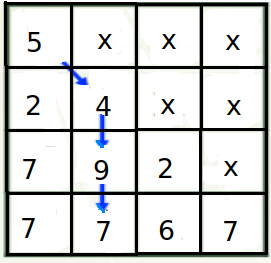
\includegraphics[width=100pt,height=100pt]{slike/dp-table-1.png}
		\caption{Primjer putanje pijuna. Ukupna vrijednost označene putanje iznosi 25.}
		\label{fig:pijun-putanja}
	\end{figure}
	
	Problem posjeduje optimalnu podstrukturu, jer optimalna putanja do polja $(i,j)$ mora sadržavati optimalnu putanju do jednog od polja iz kojih je moguće doći u $(i,j)$.
	
	Definišimo matricu $M$ tako da vrijednost $M(i,j)$ predstavlja maksimalnu sumu koja se može ostvariti na putanji od početnog polja $(0,0)$ do polja $(i,j)$.
	
	Da bismo izračunali vrijednost $M(i,j)$, posmatramo dva moguća prethodna polja:
	
	\begin{itemize}
		\item polje $(i-1,j)$;
		\item polje $(i-1,j-1)$.
	\end{itemize}
	
	Ako je pijun stigao iz jednog od tih polja, tada važi rekurzivna relacija:
	
	\begin{equation}
		M(i,j)=a_{ij}+\max\{M(i-1,j),\,M(i-1,j-1)\}.
	\end{equation}
	
	Bazni slučaj definisan je sa:
	
	\begin{equation}
		M(0,0)=a_{00}.
	\end{equation}
	
	Za pozicije koje nisu dostupne pijunu (npr. izvan granica matrice) možemo postaviti vrijednost $-\infty$, kako nikada ne bi bile odabrane kao dio optimalne putanje. 	Nakon popunjavanja matrice $M$, optimalna vrijednost rješenja dobija se kao:
	
	\begin{equation}
		\max_{0 \leq j < n} M(n-1,j),
	\end{equation}
	
	odnosno kao najveća vrijednost u posljednjem redu matrice $M$.  Na ovaj način svaki podproblem rješava se tačno jednom, pa je vremenska složenost algoritma jednaka $O(n^2)$, dok je potrebni memorijski prostor takođe $O(n^2)$.
	
\end{solution}


Implementacija ovog rješenje je data sljedećim k\^odom (pristup odozgo prema dolje).

\begin{minted}[fontsize=\footnotesize,scale=0.8]{python}
	A = None #matrica sa svim -1
	def init(n):
        
            A = [ [-1] * n for _ in range(n)  ]
            A[0][0] = M[0][0] #bazni slučaj
	
	def solve(k, l):# najbolji put od (0.0) do (k, l)
	    
	    for i in range(1, k):
	        for j in range(0, l):
	            best = A[i-1][j]  
	            if j>0:
	                best = max(best,  A[i-1][j-1])
	        A[i][j] = best + A[i][j]
	   
	    return A[k][l]

	#instanca
	M=[[4, 5, 7, 0],
    	[2, 3, 1, 3],
    	[1, 1, 3, 1],
    	[2, 3, 3, 3]
        ]	

	max_sum_path = 0
	for j in range(len(M)):
		init(len(A))
	        A = solve(len(A)-1, j)
		max_sum_path = max(max_sum_path, A[len(A)-1, j])
	
	#ispis rezultata	
	print(max_sum_path)
\end{minted}

\textit{Kompleksnost algoritma}. Funkcija \texttt{solve}() se izvršava u vremenu od $O(n^2)$   kao najzahtjevniji dio implementacije. Spoljašnja petlja se izvršava $n$ puta.  Prema tome, ukupna kompleksnost algoritma je $O(n^2 \cdot n)=O(n^3)$.

\end{solution}



\begin{example}
	Riješiti problem ruksaka primjenom dinamičkog programiranja.
\end{example}

\begin{solution}
	
	Posmatrajmo klasični problem ruksaka ($0$--$1$ ruksak). Ponovimo, neka je dato $n$ proizvoda, pri čemu proizvod $i$ ima težinu $w_i$ sa vrijednosti $p_i$,  $i=1,\ldots,n$. Kapacitet ruksaka iznosi $C$.
	
	\medskip
	
	\textit{Definisanje podproblema.} Neka $\textrm{DP}[i][j]$ čuva optimalnu vrijednost koju je moguće ostvariti korištenjem prvih $i$ proizvoda, za raspoloživi kapacitet ruksaka jednak $j$.  Dakle, podproblem je određen parom indeksa $
	(i,j), 
	i \in \{0,1,\ldots,n\}, 
	j \in \{0,1,\ldots,C\}.$
	
	\medskip
	
	\textit{Rekurzivna relacija.} Posmatrajmo podproblem $(i,j)$.	Postoje dva moguća slučaja:
	
	\begin{enumerate}
		\item Proizvod $i$ ne ulazi u optimalno rješenje. Tada je
	    $  \textrm{DP}[i][j] = \textrm{DP}[i-1][j].$
		\item Proizvod $i$ ulazi u optimalno rješenje. To je moguće samo ako je njegova težina manja ili jednaka raspoloživom kapacitetu, odnosno ako važi $w_i \leq j$. U tom slučaju ostvarujemo vrijednost $p_i$, a preostali kapacitet postaje $j-w_i$. Tada je
		$$
		\textrm{DP}[i][j] =\max\{ \textrm{DP}[i-1][j-w_i] + p_i, \textrm{DP}[i-1][j] \}.
		$$
		
	\end{enumerate}
	
	Birajući bolje od ova dva rješenja, dobijamo rekurzivnu relaciju:
	
	$$
	\textrm{DP}[i][j] =
	\begin{cases}
		\max\bigl(\textrm{DP}[i-1][j],\textrm{DP}[i-1][j-w_i] + p_i\bigr),
		& \text{ako } w_i \leq j, \\
		\textrm{DP}[i-1][j],
		& \text{ako } w_i > j.
	\end{cases}
	$$
	\medskip
	
	\textit{Bazni slučajevi.} Ako je kapacitet ruksaka jednak nuli, nijedan proizvod ne može biti odabran, pa vrijedi $
	\textrm{DP}[i][0]=0, i=0,\ldots,n.$  Takođe, ako ne razmatramo nijedan proizvod, maksimalna ostvariva vrijednost jednaka je nuli bez obzira na kapacitet: $\textrm{DP}[0][j]=0, j=0,\ldots,C.$
	
	\medskip
	
	\textit{Konačno rješenje.}	Nakon popunjavanja matrice $\textrm{DP}$, optimalna vrijednost problema nalazi se u ćeliji $
	\textrm{DP}[n][C].$	Drugim riječima, ona predstavlja najveću moguću vrijednost koju možemo smjestiti u ruksak kapaciteta $C$ razmatrajući svih $n$ proizvoda.
	
	\medskip
	
	\textit{Složenost algoritma.}  Matrica $\textrm{DP}$ sadrži $(n+1)(C+1)$ elemenata, a svaka ćelija se računa u konstantnom vremenu. Zbog toga je vremenska složenost algoritma $ O(n \cdot C),$ dok je prostorna složenost takođe $O(n \cdot C).$
	
\end{solution}
  \\
	 
	 Implementacija paradigme dinamičkog programiranja za rješavanje pro\-blema ruksaka je data narednim k\^odom.
	 
	 \begin{minted}[fontsize=\footnotesize,scale=0.8]{python}
	 def knapsack(n, C, W, p):
	 	DP = [[0 for x in range(C + 1)] for x in range(n + 1)]
	 
	 	# tabuliranje
	 	for i in range(n + 1):
	 		for j in range(C + 1):
	 			if i == 0 or j == 0:
	 				DP[i][j] = 0
	 			elif W[i-1] <= j:
	 				DP[i][j] = max(p[i-1]
	 				       +DP[i-1][j-W[i-1]],
	 				        DP[i-1][j])
	 			else:
	 				DP[i][j] = {DP}[i-1][j]
	 
	 	return DP[n][C]
	 
	 #instanca:
	 p = [60, 100, 120]
	 W = [10, 20, 30]
	 C = 50
	 n = len(p)
	 #poziv funkcije
	 print knapsack(n, C, W, p, n)
	 \end{minted}
	 
 \textit{Kompleksnost algoritma}. Najskuplji dio algoritma su dvije ugnježdene \texttt{for} petlje, koje izvršavaju $O(n \cdot C)$ iteracija. Svaka od iteracija se izvršava u konstantnom vremenu, pa je i ukupna kompleksnost algoritma jednaka $O(n \cdot C)$.
\end{solution}

Navedimo sada primjer konkretne instance problema i način popunjavanja DP tabele.

Neka je broj proizvoda $n=4$, kapacitet ruksaka $C=5$, a težine i vrijednosti proizvoda date nizovima $W=(2,3,4,5), P=(3,4,5,6).$

Formiramo matricu $\textrm{DP}$ dimenzija $(n+1)\times(C+1)$, pri čemu vrijednost $\textrm{DP}[i][j]$ predstavlja maksimalnu vrijednost koju je moguće ostvariti korištenjem prvih $i$ proizvoda i ruksaka kapaciteta $j$.

\medskip

Prvi korak sastoji se od inicijalizacije baznih slučajeva. Kako ruksak kapaciteta $0$ ne može sadržavati nijedan proizvod, vrijedi $\textrm{DP}[i][0]=0$ za sve $i$. Takođe, ako ne razmatramo nijedan proizvod, ostvarena vrijednost je jednaka nuli, pa vrijedi $\textrm{DP}[0][j]=0$ za sve $j$. Dobijamo početnu tabelu:

\begin{table}[H]
	\centering
	\begin{tabular}{|c|cc|cccccc|}\hline
		$j\rightarrow$ & Proizvod & & 0 & 1 & 2 & 3 & 4 & 5 \\ \hline
		$i=0$ & & & 0 & 0 & 0 & 0 & 0 & 0 \\
		$i=1$ & $w_1=2$ & $p_1=3$ & 0 & & & & & \\
		$i=2$ & $w_2=3$ & $p_2=4$ & 0 & & & & & \\
		$i=3$ & $w_3=4$ & $p_3=5$ & 0 & & & & & \\
		$i=4$ & $w_4=5$ & $p_4=6$ & 0 & & & & & \\ \hline
	\end{tabular}
\end{table}

\medskip

Za $i=1$ razmatramo samo prvi proizvod. Kako njegova težina iznosi $2$, nije ga moguće smjestiti u ruksak kapaciteta $0$ ili $1$. Za sve kapacitete $j\geq 2$ optimalno je uzeti taj proizvod, pa druga vrsta tabele postaje:

\begin{table}[H]
	\centering
	\begin{tabular}{|c|cc|cccccc|}\hline
		$j\rightarrow$ & Proizvod & & 0 & 1 & 2 & 3 & 4 & 5 \\ \hline
		$i=0$ & & & 0 & 0 & 0 & 0 & 0 & 0 \\
		$i=1$ & $w_1=2$ & $p_1=3$ & 0 & 0 & 3 & 3 & 3 & 3 \\
		$i=2$ & $w_2=3$ & $p_2=4$ & 0 & & & & & \\
		$i=3$ & $w_3=4$ & $p_3=5$ & 0 & & & & & \\
		$i=4$ & $w_4=5$ & $p_4=6$ & 0 & & & & & \\ \hline
	\end{tabular}
\end{table}

\medskip

Dalje popunjavamo treću vrstu ($i=2$), pri čemu su na raspolaganju prva dva proizvoda.

\begin{table}[H]
	\centering
	\begin{tabular}{|c|cc|cccccc|}\hline
		$j\rightarrow$ & Proizvod & & 0 & 1 & 2 & 3 & 4 & 5 \\ \hline
		$i=0$ & & & 0 & 0 & 0 & 0 & 0 & 0 \\
		$i=1$ & $w_1=2$ & $p_1=3$ & 0 & 0 & 3 & 3 & 3 & 3 \\
		$i=2$ & $w_2=3$ & $p_2=4$ & 0 & 0 & 3 & 4 & 4 & 7 \\
		$i=3$ & $w_3=4$ & $p_3=5$ & 0 & & & & & \\
		$i=4$ & $w_4=5$ & $p_4=6$ & 0 & & & & & \\ \hline
	\end{tabular}
\end{table}

Razmotrimo ćeliju $\textrm{DP}[2][4]$. Postoje dvije mogućnosti:

\begin{itemize}
	\item ne uzimamo drugi proizvod, pa je vrijednost jednaka $\textrm{DP}[1][4]=3$;
	\item uzimamo drugi proizvod, pa preostaje kapacitet $4-3=1$, odnosno dobijamo vrijednost $\textrm{DP}[1][1]+4=0+4=4.$
\end{itemize}

Prema tome, $\textrm{DP}[2][4]=\max\{3,4\}=4.$ Vrijednost $\textrm{DP}[2][5]=7$ dobija se uzimanjem oba proizvoda, jer vrijedi $\textrm{DP}[1][2]+4 = 3+4 = 7.$

\medskip

Popunjavanjem četvrte vrste ($i=3$) dobijamo:

\begin{table}[H]
	\centering
	\begin{tabular}{|c|cc|cccccc|}\hline
		$j\rightarrow$ & Proizvod & & 0 & 1 & 2 & 3 & 4 & 5 \\ \hline
		$i=0$ & & & 0 & 0 & 0 & 0 & 0 & 0 \\
		$i=1$ & $w_1=2$ & $p_1=3$ & 0 & 0 & 3 & 3 & 3 & 3 \\
		$i=2$ & $w_2=3$ & $p_2=4$ & 0 & 0 & 3 & 4 & 4 & 7 \\
		$i=3$ & $w_3=4$ & $p_3=5$ & 0 & 0 & 3 & 4 & 5 & 7 \\
		$i=4$ & $w_4=5$ & $p_4=6$ & 0 & & & & & \\ \hline
	\end{tabular}
\end{table}

Na primjer, za ćeliju $\textrm{DP}[3][4]$ imamo $\textrm{DP}[2][4]=4$ ako ne uzmemo treći proizvod, odnosno $\textrm{DP}[2][0]+5=5$ ako ga uzmemo. Zato je $\textrm{DP}[3][4]=\max{4,5}=5.$

\medskip

Konačno, nakon obrade četvrtog proizvoda dobijamo završnu tabelu:

\begin{table}[H]
	\centering
	\begin{tabular}{|c|cc|cccccc|}\hline
		$j\rightarrow$ & Proizvod & & 0 & 1 & 2 & 3 & 4 & 5 \\ \hline
		$i=0$ & & & 0 & 0 & 0 & 0 & 0 & 0 \\
		$i=1$ & $w_1=2$ & $p_1=3$ & 0 & 0 & 3 & 3 & 3 & 3 \\
		$i=2$ & $w_2=3$ & $p_2=4$ & 0 & 0 & 3 & 4 & 4 & 7 \\
		$i=3$ & $w_3=4$ & $p_3=5$ & 0 & 0 & 3 & 4 & 5 & 7 \\
		$i=4$ & $w_4=5$ & $p_4=6$ & 0 & 0 & 3 & 4 & 5 & 7 \\ \hline
	\end{tabular}
\end{table}

Posmatrajmo ćeliju $\textrm{DP}[4][5]$. Ako ne uzmemo četvrti proizvod, vrijednost je $ \textrm{DP}[3][5]=7.$ Ako ga uzmemo, dobijamo $\textrm{DP}[3][0]+6=6.$ Stoga je $ \textrm{DP}[4][5]=\max\{7,6\}=7.$

Kako se optimalna vrijednost problema nalazi u ćeliji $\textrm{DP}[n][C]$, zaključujemo da je optimalna vrijednost za posmatranu instancu jednaka $\textrm{DP}[4][5]=7.$  Ona se ostvaruje odabirom prvog i drugog proizvoda, čija je ukupna težina $2+3=5$, a ukupna vrijednost $3+4=7$.

 \begin{definition}
 	String $s$ je podniz stringa $s_1$ akko se $s$ može dobiti brisanjem (nula ili više)
 	karaktera iz stringa $s_1$ a čuvajući poredak ostalih karaktera. \\
 	Npr.  \texttt{acd} je podniz stringa \texttt{abbbcdef}.   Prefiks stringa $s$ dužine $k$ je podstring stringa $s$ koji se sastoji od prvih $k$ karaktera. Npr. prefiks dužine tri stringa \texttt{abbbcdef} je string \texttt{abb}. 
 	
 \end{definition}
 
\begin{example}
	(\textit{Problem najdužeg zajedničkog podniza} (eng. \emph{Longest Common Subsequence Problem} -- LCS)). Neka su data dva stringa $s_1$ i $s_2$. Potrebno je odrediti najduži string $s$ koji je podniz oba ulazna stringa.
	
	Na primjer, za stringove $s_1=\texttt{aatdccddc}$ i 
	$s_2=\texttt{agccddta} $
	jedno optimalno rješenje je $s=\texttt{accdd},$
	čija je dužina jednaka $5$.
\end{example}

\begin{solution}
	
	Definišimo podproblem parom indeksa $(i,j)$, gdje je
	$0 \leq i \leq |s_1|, 0 \leq j \leq |s_2|.
	$ 
	Podproblem označen parom $(i,j)$ odgovara određivanju dužine najdužeg zajedničkog podniza između prefiksa od $s_1$ dužine $i$ i prefiksa od $s_2$ dužine $j$.  Rješenja podproblema memorišemo u matrici $\textrm{DP}$, pri čemu vrijednost $\textrm{DP}[i][j]$ predstavlja dužinu najdužeg zajedničkog podniza pomenutih prefiksa.
	
	\medskip
	
	\textit{Rekurzivna relacija.} Posmatrajmo posljednje karaktere razmatranih prefiksa, odnosno karaktere $s_1[i-1]$ i $s_2[j-1]$. Moguća su dva slučaja.
	
	\begin{itemize}
		\item Ako je
		$s_1[i-1]=s_2[j-1],$
		tada taj karakter može biti dio optimalnog rješenja. Optimalni podniz podproblema $(i,j)$ dobija se proširivanjem optimalnog rješenja podproblema $(i-1,j-1)$ za jedan karakter. Stoga vrijedi $\textrm{DP}[i][j]=\textrm{DP}[i-1][j-1]+1.$
		
		\item Ako je $ s_1[i-1]\neq s_2[j-1],$
		tada barem jedan od ta dva karaktera neće generisati optimalno rješenje. Zbog toga razmatramo dva podproblema 
		$ (i-1,j)$ i
		$(i,j-1)$,
		odnosno izostavljamo posljednji karakter prvog ili drugog prefiksa. Optimalna vrijednost dobija se izborom boljeg od ta dva podproblema:
		$$ \textrm{DP}[i][j]
		=
		\max\{\textrm{DP}[i-1][j],\,\textrm{DP}[i][j-1]\}.
		$$
	\end{itemize}
	
	Prema tome, rekurzija ima oblik
	
	$
	\textrm{DP}[i][j]=
	\begin{cases}
		\textrm{DP}[i-1][j-1]+1, & \text{ako je } s_1[i-1]=s_2[j-1], \\
		\max\{\textrm{DP}[i-1][j],\textrm{DP}[i][j-1]\}, & \text{inače}.
	\end{cases}
	$
	
	\medskip
	
	\textit{Bazni slučajevi.} Ako je jedan od prefiksa prazan, tada zajednički podniz ne postoji, pa je njegova dužina jednaka nuli. Zbog toga vrijedi  $\textrm{DP}[i][0]=0,
	  0\leq i\leq |s_1|,$ i $
	\textrm{DP}[0][j]=0,
	0\leq j\leq |s_2|.$
	
	\medskip
	
	Nakon popunjavanja matrice $\textrm{DP}$, dužina najdužeg zajedničkog podniza nalazi se u ćeliji $\textrm{DP}[|s_1|][|s_2|].$ Sam podniz može se rekonstruisati prolaskom unazad kroz matricu, počevši od pozicije $(|s_1|,|s_2|)$ i prateći odluke koje su dovele do optimalne vrijednosti.
	
\end{solution}

	    
	 Implementacija paradigme dinamičkog programiranja za rješavanje LCSP je data narednim k\^odom. 
 \begin{minted}[fontsize=\footnotesize,scale=0.8]{python}
	    	
	     def LCS(s1, s2): #tabuliranje
	    	      
	    	  if len(s1)==0 or len(s2)==0:
	    	     return 0
	    	     
	    	  DP = [ [0]*(len(s2)+1) for _ in range(len(s1)+1)]
	              for i in range(1, len(s1)+1):
	    	      for j in range(1, len(s2)+1):
	    		     if s1[i-1] == s2[j-1]: 
	    		         DP[i][j] = DP[i-1][j-1] + 1
	    		     else:
	    		         DP[i][j] = max(DP[i-1][j], DP[i][j-1])
	    	  return DP[len(s1)][len(s2)]        
	    		           
	    	      
	     #instanca:
	     s1 = "abcdcdcdaa"
	     s2 = "abbaabcccddd"
	     #poziv DP metoda
	     lcs = LCS(s1, s2)
	     print("Duzina LCS-a je: ", lcs)     
 \end{minted}
	     Primijetimo da implementacija koristi princip odozdo-nagore.
	     
	     \textit{Kompleksnost algoritma}. Dvije \texttt{for}-petlje  izvršavaju ukupno $O(|s_1|\cdot |s_2|)$ iteracija. Svaka od iteracija se izvršava u konstantnom vremenu, pa je shodno tome ukupno vrijeme izvršavanja algoritma jednako $O(|s_1| \cdot |s_2|)$. Ako je $n = \max\{|s_1|, |s_2|\}$, dobija se kvadratna $O(n^2)$ kompleksnost. 
	     
	     %\begin{figure}[H]
	     %	\centering
	     %	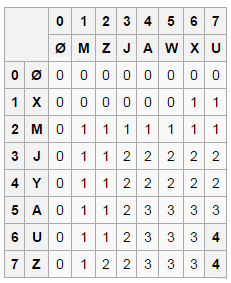
\includegraphics[width=150pt,height=150pt]{slike/dp-lcs-table.png}
	     %	\caption{DP matrica za dva stringa $s_1=$\texttt{MZJAWXU} i $s_2=$\texttt{XMJYAUZ}. Rješenje je dužine 4 (pogledati donji desni ugao matrice). }
	     %\end{figure}
     
     \begin{table}
     	  \centering
     	  \begin{tabular}{cc|cccccccc}
     	  	& & 0&1 &2 &3 &4 &5 &6 &7   \\
     	  
     	  	& & $\emptyset$&\texttt{M} &\texttt{Z} &\texttt{J} &\texttt{A} &\texttt{W} &\texttt{X} &\texttt{U}  \\ \hline \hline
     	  	
     	  	0&$\emptyset$ &0& 0& 0&  0&0 &0 & 0   & 0 	   \\
     	  	1& \texttt{X}& 0& 0& 0& 0& 0& 0&  1  & 1                \\	
     	  	2& \texttt{M}& 0& 1& 1& 1& 1& 1&  1  & 1                \\	
     	  	3& \texttt{J}& 0& 1& 1& 2& 2& 2&  2  & 2                \\	
     	  	4& \texttt{Y}&0 & 1& 1& 2& 2& 2&  2  & 2                 \\	
      	  	5& \texttt{A}& 0& 1& 1& 2& 3& 3&  3  & 3                \\	
      	  	6& \texttt{U}& 0& 1& 1& 2& 3& 3&  3  & 4                \\	
      	  	7& \texttt{Z}& 0& 1& 2& 2& 3& 3&  3  & 4                \\	 \hline \hline
     	  \end{tabular}
 	 \caption{DP matrica za LCSP dva stringa $s_1=$\texttt{MZJAWXU} i $s_2=$\texttt{XMJYAUZ}. Rješenje je dužine 4 (pogledati donji desni ugao matrice). }  \label{tab:dp-lcs-example} 
 	\end{table}
\end{solution}

%https://www.programiz.com/dsa/longest-common-subsequence ==> primjer tabele sa rješenjem...

\begin{example} \textbf{Problem sume podskupa} (eng. \emph{Subset Sum Problem}). Neka je dat niz od $n$ nenegativnih cijelih brojeva i ciljna vrijednost \textit{sum}. Potrebno je odrediti da li postoji podskup elemenata datog niza čiji je zbir jednak vrijednosti \textit{sum}.
\end{example}

\begin{solution}
	
	Posmatrajmo primjer u kojem je $
	niz=[1,7,8,2,6]
	$ i  $sum=9.$
	
		Odgovor je pozitivan, jer podskup ${1,2,6}$ ima zbir jednak $9$.
	
	\medskip
	
	Da bismo riješili problem dinamičkim programiranjem, definišimo podproblem određen parom indeksa
	
	$$
	(i,j),
	0 \leq i \leq n,
	0 \leq j \leq sum.
	$$
	
	Podproblem $(i,j)$ odgovara pitanju:
	
	\begin{quote}
		Da li među prvih $i$ elemenata niza postoji podskup čiji je zbir jednak $j$?
	\end{quote}
	
	Rješenja podproblema memorišemo u matrici $\textrm{DP}$, gdje je
	
	$$
	\textrm{DP}[i][j]=
	\begin{cases}
		True, & \text{ako takav podskup postoji},\\
		False, & \text{inače}.
	\end{cases}
	$$
	
	\medskip
	
	\textit{Rekurzivna relacija.} 	Posmatrajmo podproblem označen parom $(i,j)$ i element $niz[i-1]$. Postoje dva moguća slučaja.
	
	\begin{itemize}
		\item {Element $niz[i-1]$ pripada rješenju.}
		
		U tom slučaju preostali elementi moraju formirati zbir $j-niz[i-1].$	Stoga vrijedi $\textrm{DP}[i][j] = \textrm{DP}[i-1][j-niz[i-1]],$
		pod uslovom da je $
		j \geq niz[i-1].$
		
		\item {Element $niz[i-1]$ ne uzimamo u rješenje.} Tada se problem svodi na prvih $i-1$ elemenata:
		$ \textrm{DP}[i][j] = \textrm{DP}[i-1][j].$
		
	\end{itemize}
	
	Pošto je dovoljno da bude zadovoljen bilo koji od ova dva slučaja, dobijamo rekurziju
	
	$$
	\textrm{DP}[i][j]=
	\textrm{DP}[i-1][j] \vee \textrm{DP}[i-1][j-niz[i-1]],$$
	ako je $j \geq niz[i-1].$	U suprotnom, element ne može biti dio rješenja, pa vrijedi $\textrm{DP}[i][j] =	\textrm{DP}[i-1][j].$
	
	\medskip
	
	\textit{Bazni slučajevi.}  	Zbir $0$ uvijek možemo ostvariti izborom praznog podskupa, pa vrijedi $
	\textrm{DP}[i][0]=True, 
	0\leq i\leq n.$ 	S druge strane, ako ne raspolažemo niti jednim elementom, nijedan pozitivan zbir ne može biti formiran $ \textrm{DP}[0][j]=False, 1\leq j\leq sum.
	$
	
	\medskip
	
	Nakon popunjavanja matrice $\textrm{DP}$, odgovor na početni problem nalazi se u ćeliji $\textrm{DP}[n][sum].$
	
	Ako je vrijednost ove ćelije \textit{True}, postoji podskup čiji je zbir jednak zadanoj vrijednosti \textit{sum}; u suprotnom takav podskup ne postoji.
	
\end{solution}

   
    Implementacija paradigme dinamičkog programiranja za rješavanje Pro\-blema \emph{sume podskupa} je data narednim k\^odom. 
   
   \begin{minted}[fontsize=\footnotesize,scale=0.8]{python}
   	  def sum_array(niz, suma):
   	      #tabulation:
   	      DP = [[False] * (suma +1) for _ in range(len(niz) + 1) ]
   	      for i in range(len(niz)+1):
   	          DP[i][0] = True
   	      
   	      for i in range(1, len(niz)+1):   
   	          for j in range(1, suma+1):
   	              if j >= niz[i-1]:
   	                 DP[i][j] = DP[i-1][j-niz[i-1]] or DP[i-1][j]
   	              else:
   	                 DP[i][j] = DP[i-1][j]
   	                 
   	      return DP[len(niz)][suma]
   	  
   	  #instanca:
   	  niz = [3, 34, 4, 12, 5, 2]
   	  suma = 9
   	  postoji = sum_array(niz, suma)
   	  print("Postoji podskup sa sumom" if postoji else  
   	        "Ne postoji podskup sa sumom")
   \end{minted}
\end{solution}
Primijetimo da smo dinamičko programiranje implementirali pomoću pristupa \textit{odozdo prema gore} (tabuliranje). 

Implementirajmo sada dinamičko programiranje za ovaj problem pristupom \textit{odozgo prema dolje}.

   \begin{minted}[fontsize=\footnotesize,scale=0.8]{python}
	def init(niz, suma):
		global DP
		DP = [[-1] * (suma + 1) for _ in range(len(niz) + 1) ]
	
	
	def sum_array_top_down(niz, suma, i, j, DP = [ ]):
	
		if DP[i][j] != -1:
			return DP[i][j]
	
		if j == 0:
			DP[i][0] = True
			return True 
		if i == 0: 
			DP[0][j] = False
			return False
		#recursion: 
		if j >= niz[i-1]:  
			DP[i][j] = sum_array_top_down(niz, suma, i-1, j, DP) or
			sum_array_top_down(niz, suma, i-1, j-niz[i-1], DP)
			return DP[i][j]
		else:
			DP[i][j] = sum_array_top_down(niz, suma, i-1, j, DP)
			return DP[i][j]
\end{minted}  

\textit{Kompleksnost algoritma}. Broj iteracija koje se izvršavaju je jednak $O(n \cdot sum)$. Svaka iteracija se izvršava u konstantnom vremenu, pa je i ukupna kompleksnost algoritma jednaka  $O(n \cdot sum)$. Dakle, ako je vrijednost \emph{sum} ogromna, ekponencijalno velika u odnosu na veličinu niza, ovakav algoritam će biti neefikasan. 

\begin{example}
	(\textit{Problem rezanja štapa}). Dat je štap dužine $n$ i niz cijena \textit{price}, pri čemu \textit{price}$[i-1]$ predstavlja cijenu štapa dužine $i$, za svako $1 \leq i \leq n$.\\ 
	
	Potrebno je odrediti način rezanja štapa na manje dijelove tako da ukupan ostvareni profit bude maksimalan.
	
\end{example}

\begin{solution}
	
	Posmatrajmo primjer instance problema date sa 
	$$price = [1,5,8,9,10,17,17,20].$$ 
	Pretpostavimo da je dužina štapa $n=4.$	Ako se štap ne reže, ostvaruje se profit jednak $9$. Međutim, ako ga podijelimo na dva dijela dužine $2$, dobijamo profit $
	5+5=10,
	$ što predstavlja bolje (u ovom slučaju optimalno) rješenje za tu instancu.
	
	\medskip
	
	Da bismo problem riješili dinamičkim programiranjem, definišimo podproblem dužinom štapa $i$, gdje je $
	0 \leq i \leq n.
	$
	
	Neka $\textrm{DP}[i]$ označava maksimalni profit koji se može ostvariti rezanjem štapa dužine $i$. Vrijednost $\textrm{DP}[i]$ memorišemo u nizu $\textrm{DP}$ na poziciji $i$.
	
	\medskip
	
	\textit{Rekurzivna relacija.} Posmatrajmo štap dužine $i$. Podijelimo ovaj štap na dio dužine $k$, gdje je $ 1 \leq k \leq i.$ Na taj način štap dijelimo na:
	
	\begin{itemize}
		\item dio dužine $k$, čija je vrijednost $price[k-1]$;
		\item preostali dio dužine $i-k$, čiji je optimalni profit jednak $\textrm{DP}[i-k]$.
	\end{itemize}
	
	Za svaku moguću vrijednost $k$ dobijamo kandidatsko rješenje $price[k-1] + \textrm{DP}[i-k].$  Optimalna vrijednost za štap dužine $i$ dobija se izborom najboljeg među svim mogućim prvim rezovima:
	
	$$
	  \textrm{DP}[i] =
	  \max_{1 \leq k \leq i}
	  \left\{
		price[k-1] + \textrm{DP}[i-k]
		\right\}.
	$$
	
	\medskip
	
	\textit{Bazni slučaj.} Štap dužine $0$ nema vrijednost, pa vrijedi $\textrm{DP}[0]=0.$
	
	\medskip
	
	Nakon popunjavanja niza $\textrm{DP}$, optimalna vrijednost početnog problema nalazi se u ćeliji $
	\textrm{DP}[n].$ 	Vrijednost $\textrm{DP}[n]$ predstavlja maksimalan profit koji se može ostvariti rezanjem štapa dužine $n$.
	
	\medskip
	
	\textit{Vremenska složenost.}	Za svaku dužinu $i$ razmatra se najviše $i$ mogućih pozicija prvog reza. Ukupan broj operacija jednak je $	\sum_{i=1}^{n} i =
	\frac{n(n+1)}{2},
	$  pa je vremenska složenost algoritma $O(n^2).$  Prostorna složenost iznosi $O(n),$ jer se koristi jednodimenzionalni niz $\textrm{DP}$ veličine $n+1$.
	
\end{solution}


 Implementacija paradigme dinamičkog programiranja za rješavanje problema  rezanja štapa je data narednim k\^odom. 
 
 \begin{minted}[fontsize=\footnotesize,scale=0.8]{python}
	def stick_cut(d, price):

		DP = [-1] * (d+1)  #init
		DP[0], DP[1] = 0, price[0]

		for i in range(2, d+1):
			for k in range(1, i+1):
				if DP[i] < DP[i-k] + price[k-1]: 
					DP[i] =  DP[i-k] + price[k-1]
		return DP[d]       
     
     #instanca
     d = 4
     price = [1, 5, 8, 9, 10, 17, 17, 20] 
     max_profit = stick_cut(d, price)     
     #poziv
     print(max_profit)
 \end{minted} 
\textit{Napomena}. Pogledajmo drvo rekurzije koje se kreira algoritmom grube sile na Slici~\ref{fig:brute-force-stick-cut}  pri rješavanju problema rezanja štapa za $d=4$. Ovaj pristup enumeriše sva moguća rješenja za rezanje štapa dužine $d=4$. Prvo uzima cio štap u razmatranje (i njegovu cijenu), zatim otkida dio štapa dužine 1, dok se ostatak štapa (dužine 3) rješava (dijeli) rekurzivno itd. Kompletno rješenje dobijamo u listovima stabla (označeni sa 0). 
\begin{center}
	\begin{figure}[H]
		\centering
		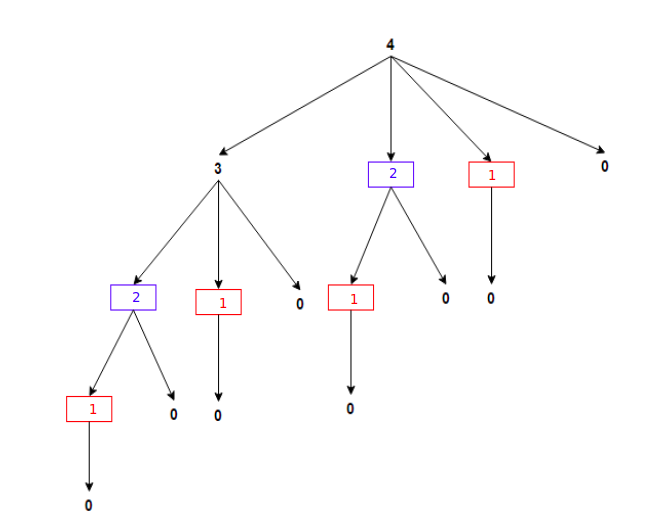
\includegraphics[width=300pt,height=230pt]{slike/brute-force-cutting-stick.png}
		
		\caption{Drvo grananja paradigme grube sile za rješavanje problema rezanja štapa.}\label{fig:brute-force-stick-cut}
	\end{figure}
\end{center}



  Npr. put koji posjećuje čvorove sa oznakama 4 $\rightarrow$ 3 $\rightarrow$ 2 $\rightarrow$ 1 $\rightarrow$ 0, odgovara rješenju u kojem se štap siječe na 4 manja štapa dužine 1 (cijene $4 \times price[0]$). Slično, za put koji posjećuje čvorove sa oznakama 4 $\rightarrow$ 3 $\rightarrow$ 1 $\rightarrow$ 0, odgovara rješenju u kojem se štap sječe na dva manja štapa dužine 1, te jedan dužine 2 (cijene $2 \times price[0] + price[1]$).   
  
   Jasno se vidi da se podproblemi isprepliću, tj. da se, npr. rješavanje problema štapa dužine dva računa više (dva) puta. U slučaju dinamičkog programiranja implementiran  pristupom odozgo prema dolje, stablo će biti značajno redukovano, jer neće postojati rekalkulacije istih podproblema (dakle, nema identičnih kopija podstabala u DP stablu). 
 

\section*{Zadaci}

\begin{enumerate}
	\item Riješiti problem trgovačkog putnika pomoću algoritamske paradigme grube sile.
	\item Riješiti problem ruksaka pomoću algoritamske paradigme grube sile.
	\item Dati  su brojevi  $0 \leq  M  <  N  \leq  1,000,000$. Odrediti  najmanji  broj  sastavljen  samo  od 
	neparnih cifara, koji pri dijeljenju sa $N$ daje ostatak $M$. Ukoliko traženi broj ne postoji, vratiti $−1$. 
	
	 \item Neka su dati prirodni brojevi $n$, koji označava broj promjenljivih, i $s$, koji označava sumu promjenljivih. Uz
pomoć rekurzivnih algoritama napisati program koji pronalazi sva moguća rješenja
za promjenljive  kojih ima $n$ i  čija   suma treba biti jednaka $ s$. 

\textit{Instanca}: $n = 5, s = 4$;
\textit{Rješenje}: 70. \\
\textit{Napomena}.
Instanca predstavlja jednačinu $x_1 + x_2 + x_3 + x_4 + x_5 = 4, x_i \in \mathbb{N}$. 
Sva moguća rješenja su:
$(1\ 1\ 1\ 1\ 0), (1\ 0\ 1\ 1\ 1), (0\ 1\ 1\ 1\ 1), \ldots ,$ $(2\ 1\ 0\ 0\ 1), \ldots , (2\ 2\ 0\ 0\ 0)$ itd.
	%pohlepni algoritmi (dva zadatka) 
	%https://www.geeksforgeeks.org/minimum-product-subset-array/
	\item Pronaći podskup elemenata niza tako da  proizvod elemenata u podskupu bude minimalan. Koristiti paradigmu pohlepnih algoritama.\\
	 \textit{Instanca}: $niz = [ -1, -1, -2, 4, 3]$; \textit{Rješenje}:  -24 ($=(-2 )\cdot (-1) \cdot (-1) \cdot 4 \cdot 3$). 
	
	%https://www.geeksforgeeks.org/greedy-algorithm-egyptian-fraction/
	\item Svaki pozitivan razlomak možemo predstaviti kao zbir jedi\-nstvenih jediničnih razlomaka. Razlomak je jedinični ako je brojnik 1, a nazivnik pozitivan cijeli broj; npr. $1/3$ je jedinični razlomak. Npr. $2/3= 1/2 + 1/6, 3/7=1/3 + 1/11 + 1/231.$   Uz pomoć paradigme pohlepnih algoritama, za proizvoljan razlomak, naći jedinične razlomke koje u zbiru daju taj razlomak.  
	
	
	\item Riješiti problem nalaska najdužeg zajedničkog podniza dva stringa pomoću dinamičkog programiranja pristupom odozgo prema dolje. 
	
	\item U ulazu je dat niz brojeva.  Konstruisati algoritam dinamičkog programi\-ranja koji daje odgovor na pitanje li postoji particionisanje niza na dva (disjunktna) skupa tako da je zbir elemenata u obje particije jednak.
	\item Implementirati metod dinamičkog programiranja  za problem rezanja štapa koristeći pristup odozgo prema dolje.
	
	\item Neka su u ulazu data dva stringa $s_1$ i $s_2$. Uz pomoć dinamičkog programi\-ranja, pronaći najkraći string $s$ tako da
	su stringovi $s_1$ i $s_2$ podnizovi stringa $s$.
	\item  Data  je riječ i riječnik (skup riječi). Ispitati da li se riječ može podijeliti na segmente (podstringove) tako da oni pripadaju riječniku. \\
	
	\textit{Instanca}: $$dict = \{\texttt{this}, \texttt{th}, \texttt{is}, \texttt{famous}, \texttt{Word}, \texttt{break}, \texttt{b}, \texttt{r}, \texttt{e}, \texttt{a}, \texttt{k},	\texttt{br}, \texttt{bre}, \texttt{brea}, \texttt{ak}, \texttt{problem} \} $$ te   $$word = \texttt{Wordbreakproblem}.$$  
	\textit{Rješenje}: \texttt{Word break problem},  kao jedno od rješenja.
	
	\item Neka je dat pravougaonik dimenzija $N\times M$. Pretpostavimo da je na raspolaganju beskonačan broj pločica
	formata $2^i \times 2^i$, $i = 0, 1, 2, 3, \ldots $. 
	
	Napisati program koji rekurzivno pronalazi minimalan broj pločica koji je potreban da bi se
	popločao pravougaonik datih dimenzija.
	
	\textit{Instanca}:  $N = 6, M=5$;	\textit{Rješenje}: 9 (pločica) -- vidjeti narednu sliku. %~\ref{fig:plocice}. 
	
	\begin{figure}[H]
	    \centering
		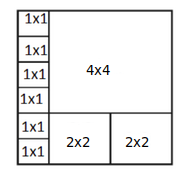
\includegraphics[width=120pt,height=100pt]{slike/plococe-dp-zadatak.png}
		\label{fig:plocice}
		\caption{Optimalno pokrivanje ploče 6 $\times$ 5}
	\end{figure}

\item Napisati program koji generiše sve mogućnosti da se stavi $+$ ili $-$ ili niti jedna od ove dvije opcije između brojeva $1,2,\ldots,9$ (ovim redom) tako da se kao rezultat izvršenja operacija dobije vrijednost 100. Npr. jedno takvo rješenje je $1 + 2 + 3 - 4 + 5 + 6 + 78 + 9 = 100$.
 
 \item Za dva stringa, napisati program koji ispisuje najkraći niz umetanja i brisanja karaktera u prvi string čijom se primjenom  dobija drugi string.
\end{enumerate}